\documentclass[journal, onecolumn]{IEEEtran}

\usepackage{graphicx}
\usepackage{amsmath}
\usepackage{amsfonts}
\usepackage{cite}
\usepackage{float}
\usepackage{subcaption}
\usepackage{url}
\usepackage{booktabs}
\usepackage{multirow}
\usepackage{placeins}   % provides \FloatBarrier

% --- Reduce white gaps around floats ---
\setlength{\intextsep}{8pt plus 2pt minus 2pt}     % space above/below in-text floats
\setlength{\floatsep}{8pt plus 2pt minus 2pt}       % between consecutive floats
\setlength{\textfloatsep}{10pt plus 2pt minus 4pt}  % between float and text
\setlength{\abovecaptionskip}{6pt}                   % space above caption
\setlength{\belowcaptionskip}{2pt}                   % space below caption
\renewcommand{\topfraction}{0.9}      % max fraction of page for top floats
\renewcommand{\bottomfraction}{0.9}   % max fraction of page for bottom floats
\renewcommand{\textfraction}{0.1}     % min fraction of page for text
\renewcommand{\floatpagefraction}{0.7}% min fraction before a float-only page

\title{MTAN-Lite: Lightweight Multi-Task Attention Network for Real-Time Dense Scene Understanding}

\author{
\IEEEauthorblockN{S. A. Sajidha\textsuperscript{1}, Siddhartha Mallavolu\textsuperscript{1}, and Puvvada V. N. S. N. Kedhar\textsuperscript{2}}
\IEEEauthorblockA{\textsuperscript{1}School of Computer Science and Engineering, Vellore Institute of Technology, Chennai, India\\
\textsuperscript{2}School of Electronics Engineering, Vellore Institute of Technology, Chennai, India\\
Email: sajidha.s@vit.ac.in, sidmallaofficial@gmail.com, kedharpuvvada@gmail.com}
}

\begin{document}

\maketitle

\begin{abstract}
Dense scene understanding is important for applications like assistive navigation, especially considering that roughly one-sixth of the global population has some form of visual impairment~\cite{messaoudi2022review}. Such applications need to perceive obstacle distances, walkable regions, and surface geometry all at once from visual input. Existing solutions tend to rely on costly active sensors like LiDAR or RGB-D cameras, or they use multiple separate deep learning models that together exceed the memory and speed budgets of mobile devices. Multi-task learning (MTL) can jointly predict depth, semantics, and surface normals in one forward pass, but current MTL architectures use heavy backbones with tens to hundreds of millions of parameters, which makes them impractical for edge deployment. In this paper, we present MTAN-Lite, a lightweight version of the Multi-Task Attention Network where we swap out the SegNet encoder for MobileNetV3-Large and redesign the attention modules using reduced-dimensionality channel-wise bottlenecks with pointwise ($1 \times 1$) convolutions. The model jointly predicts monocular depth, semantic segmentation, and surface normals from a single RGB image. On Cityscapes at $512\times1024$ resolution, MTAN-Lite gets 70.1\% mIoU (19-class), 84.9\% $\delta_1$ depth accuracy, and 49.1$^\circ$ surface normal MAE using only 6.2M parameters (81\% fewer than MTAN), while running at 39.6 FPS on an NVIDIA GTX 1650 with 102 MB GPU memory. We also evaluate on NYUv2 with real sensor ground truth and obtain 51.7\% mIoU (13-class), 0.621m RMSE, and 23.9$^\circ$ normal MAE, which beats MTAN and MTI-Net on segmentation with 3 to 5$\times$ fewer parameters. To our knowledge, MTAN-Lite is the first model under 10M parameters that does three-task dense prediction on both an outdoor and an indoor benchmark.
\end{abstract}

\begin{IEEEkeywords}
Real-time perception, multi-task learning, MTAN, lightweight deep learning, assistive navigation, MobileNetV3, surface normal estimation, Cityscapes, NYUv2.
\end{IEEEkeywords}

\section{Introduction}

Understanding a scene in terms of depth, semantics, and surface geometry at the same time is critical for navigation systems, whether they are meant for autonomous vehicles or assistive devices for visually impaired users. About one-sixth of the world's population deals with some degree of visual impairment, yet affordable assistive tools remain hard to come by, particularly in low- and middle-income regions~\cite{messaoudi2022review}. Most current assistive systems use expensive active sensors like LiDAR, stereo cameras, or RGB-D setups, which add significant cost, weight, and power requirements that make wearable deployment difficult~\cite{abidi2024review}. The alternative was to run separate deep learning models for each task, but that needed multiple inference passes and more memory than what typical mobile processors can handle. A simple monocular RGB camera can capture visual input at a very low cost, but extracting depth, semantics, and surface geometry from a single image in real-time requires a multi-task architecture that is small enough to run on constrained hardware. Bridging the gap between what the model needs to do and what the hardware can support is the primary problem we address in this paper.

Each individual perception tasks have made good progress on its own, but none of them was enough by itself. Monocular depth estimation has improved a lot because of the transformer architectures and large scale pretraining~\cite{ranftl2021dense, yang2024depthanything}, but depth maps on their own tend to struggle with texture-less regions, reflective surfaces, and shadows. Semantic segmentation gives useful object level information, and models like SegFormer~\cite{xie2021segformer} and DeepLabv3+~\cite{chen2018deeplabv3plus} work well on urban driving datasets, but class labels alone do not tell you anything about surface orientation or how navigable a region is. Surface normal estimation helps with depth consistency and reasoning about boundaries~\cite{bansal2016normal}, but it is rarely combined with the other two tasks in a single model. On its own no single task gives you enough for reliable scene understanding.

Multi task learning addresses this by predicting several outputs from shared features, which saves computation and can actually help each task learn better. MTAN~\cite{liu2019mtan} showed that task-specific soft attention over a shared encoder works well for dense prediction. After that, MTI-Net~\cite{vandenhende2020mti} added multi-scale task interaction, and PAD-Net~\cite{xu2018padnet} used prediction-and-distillation modules for cross-task refinement. Most recent work has gone in the direction of heavier models like InvPT~\cite{ye2022invpt} which uses ViT-Large, MTMamba~\cite{lin2024mtmamba} which uses Mamba blocks on a Swin-Large backbone, and DenseMTL~\cite{lopes2023densemtl} evaluated cross-task attention on Cityscapes for segmentation, depth, and normals. The problem is that all these methods need large backbones (ResNet-50, HRNet, Swin-Large, Vision Transformers) with tens to hundreds of millions of parameters which rules them out for real-time use on low-power hardware.

Even with all this progress, there is still a clear gap when it comes to deployment. The original MTAN was only tested on Cityscapes at 128$\times$256 with 7 semantic classes, which is too low resolution to pick up fine grained categories like poles, traffic lights, and cyclists that matter for navigation. Its SegNet backbone has 32.4M parameters, so scaling it to higher resolution or adding more tasks to it is not really feasible on mobile GPUs. The newer methods like InvPT ($>$300M parameters), MTMamba (308 MB model size), and LAKNet~\cite{laknet2025} (38.6M parameters) push the numbers higher but they are even less deployable. As far as we can tell nobody has done lightweight three-task learning (full 19-class segmentation, depth, and surface normals) on Cityscapes at real-time speed with a model that could actually run on edge hardware.

To address this, we propose \textbf{MTAN-Lite}, a lightweight multi-task attention network. We replace the standard encoder with MobileNetV3-Large and use reduced-dimensionality channel-wise attention based on pointwise ($1 \times 1$) convolutions. The model predicts monocular depth, 19-class semantic segmentation, and surface normals from a single RGB input. At just 6.2M parameters, it achieves 70.1\% mIoU, 84.9\% $\delta_1$ depth accuracy, and 49.1$^\circ$ surface normal MAE on Cityscapes, running at 39.6 FPS on an NVIDIA GTX 1650. We also evaluate on NYUv2~\cite{silberman2012nyu}, where it reaches 51.7\% mIoU, beating both MTAN and MTI-Net with 3 to 5$\times$ fewer parameters.

\noindent \textbf{Key contributions:}
\begin{itemize}
    \item We build a lightweight MTAN variant with MobileNetV3-Large and reduced-dimensionality channel-wise attention that cuts parameters by 81\% compared to the original MTAN, while still achieving competitive multi-task accuracy.
    \item To the best of our knowledge, this is the first time joint 19-class segmentation, depth estimation, and surface normal prediction has been evaluated on Cityscapes using a lightweight model. We derive surface normal pseudo-ground-truth from stereo disparity using geometric cross-product computation.
    \item We validate on NYUv2 with real sensor ground truth and achieve 51.7\% mIoU, outperforming both MTAN and MTI-Net with 3 to 5$\times$ fewer parameters. This shows the architecture works across outdoor and indoor settings.
    \item Our ablation study shows that multi-task learning gives a 3.3\% mIoU boost over training segmentation alone, confirming that cross-task feature sharing helps even at this parameter budget.
    \item The model runs at 39.6 FPS using only 102 MB of GPU memory which makes it viable for deployment on resource constrained devices.
\end{itemize}

% === RELATED WORK ===
\section{Related Work}

\subsection{Monocular Depth Estimation}

Estimating dense depth from a single RGB image is a fundamentally ill-posed problem since there are no explicit geometric constraints to work with. Ranftl et al.~\cite{ranftl2021dense} introduced the Dense Prediction Transformer (DPT), which uses Vision Transformer encoders to get globally coherent depth maps. Depth Anything~\cite{yang2024depthanything} showed that semi-supervised pretraining on over 60 million unlabeled images gives good zero-shot generalization, though it needs a lot of compute. AdaBins~\cite{bhat2021adabins} takes a different approach with adaptive binning, splitting the depth range into learned intervals using a mini-ViT module. These methods get impressive results, but they are all single-task models with 25M to over 100M parameters, and they do not give you any semantic or geometric context for navigation.

\subsection{Semantic Segmentation}

DeepLabv3+~\cite{chen2018deeplabv3plus} introduced atrous separable convolutions with an encoder-decoder structure, and lightweight variants using MobileNetV2 achieve approximately 72.5\% mIoU on Cityscapes. SegFormer~\cite{xie2021segformer} replaced convolution-based decoders with a hierarchical Mix Transformer encoder and all-MLP decoder, achieving 71.9\% mIoU on Cityscapes validation with the B0 variant at 3.8M parameters and 48 FPS. However, these architectures are designed exclusively for segmentation and do not produce depth or surface geometry information.

\subsection{Surface Normal Estimation}

Surface normal prediction recovers per-pixel orientation vectors describing local surface geometry. Bansal et al.~\cite{bansal2016normal} demonstrated that normals serve as an effective intermediate representation bridging 2D features and 3D understanding. Bae and Davison~\cite{bae2024dsine} proposed DSINE, incorporating per-pixel ray direction as an inductive bias and estimating normals through iterative relative rotation, achieving strong generalization from only 160K training images. DSINE also provides utility functions for converting depth maps to normals via geometric cross-product computation. In our work, we use this depth-to-normal conversion (not the neural network) to generate pseudo-ground-truth normals from Cityscapes stereo disparity.

\subsection{Multi-Task Dense Prediction}

Multi-task learning trains a single model for multiple prediction tasks, exploiting shared representations to improve generalization and reduce computation. MTAN~\cite{liu2019mtan} introduced task-specific soft attention masks on a shared SegNet encoder, but was evaluated on Cityscapes with only 7-class segmentation and depth at 128$\times$256 resolution, without surface normals. PAD-Net~\cite{xu2018padnet} extended this by distilling cross-task information through spatial attention on initial per-task predictions. MTI-Net~\cite{vandenhende2020mti} demonstrated that task affinity varies across scales, proposing multi-scale distillation with HRNet-18 and ResNet-18 FPN backbones.

Recent approaches adopt heavier architectures for richer cross-task interaction. InvPT~\cite{ye2022invpt} uses ViT-Large with inverted pyramid UP-Transformer blocks. MTMamba~\cite{lin2024mtmamba} replaces attention with Mamba-based self-task (STM) and cross-task (CTM) blocks using a Swin-Large encoder, achieving 55.82\% mIoU on NYUv2 at 308 MB model size. DenseMTL~\cite{lopes2023densemtl} evaluates segmentation, depth, and normals on Cityscapes using HRNet-18, with normals derived from stereo depth similarly to our approach.

All of these methods depend on large backbones with many millions of parameters, and none of them are really designed with edge deployment or real-time speed as a priority. Our work tries to fill this gap: we build a three-task network on top of MobileNetV3-Large with only 6.2M parameters total, and show that it can run in real time on both the 19-class Cityscapes and 13-class NYUv2 benchmarks.

% === PROPOSED METHOD ===
\section{Proposed Method}

\subsection{Architecture Overview}

MTAN-Lite follows a shared-encoder, task-specific-decoder paradigm for joint prediction of monocular depth, semantic segmentation, and surface normals from a single RGB input. The architecture comprises three modules: (1) a shared MobileNetV3-Large encoder that extracts multi-scale features, (2) task-specific channel-wise attention modules that modulate the deepest encoder features independently for each task, and (3) three parallel decoders with skip connections that progressively upsample to full resolution. Fig.~\ref{fig:architecture} illustrates all three modules and Table~\ref{tab:params} summarizes the parameter distribution.

\begin{figure}[!htbp]
\centering
% --- Module 1: Encoder ---
\begin{subfigure}[b]{0.85\columnwidth}
    \centering
    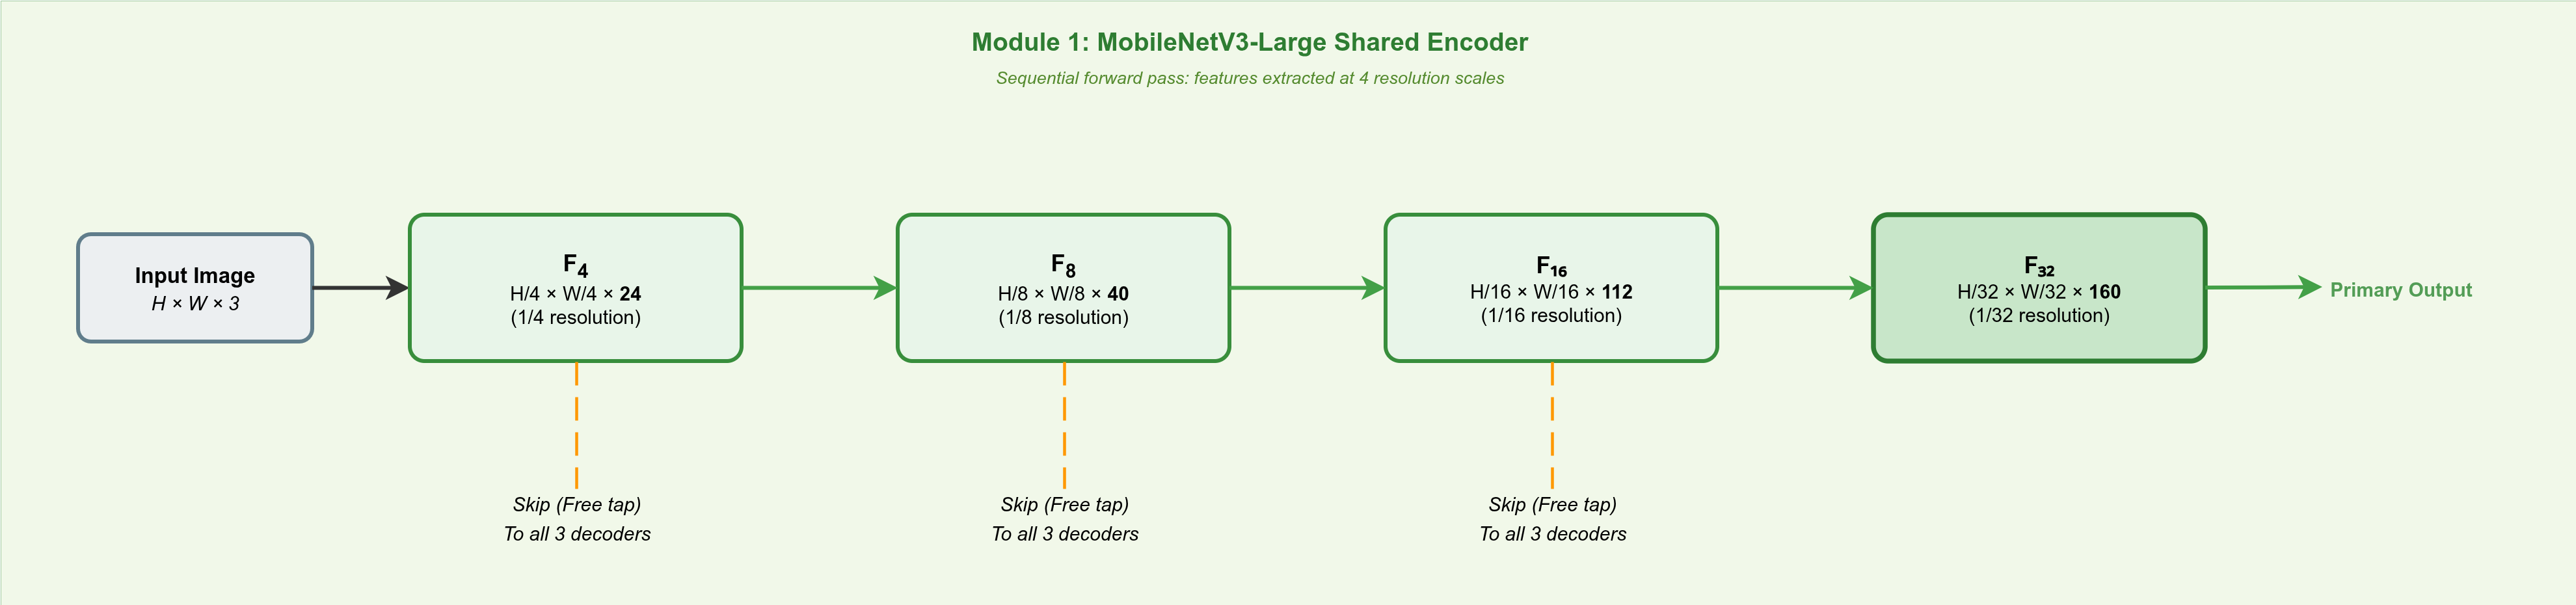
\includegraphics[width=\linewidth]{figures/arch_encoder.png}
    \caption{Module 1: MobileNetV3-Large shared encoder with feature taps at four resolution scales.}
    \label{fig:arch_encoder}
\end{subfigure}

\vspace{2pt}

% --- Module 2: Attention ---
\begin{subfigure}[b]{0.85\columnwidth}
    \centering
    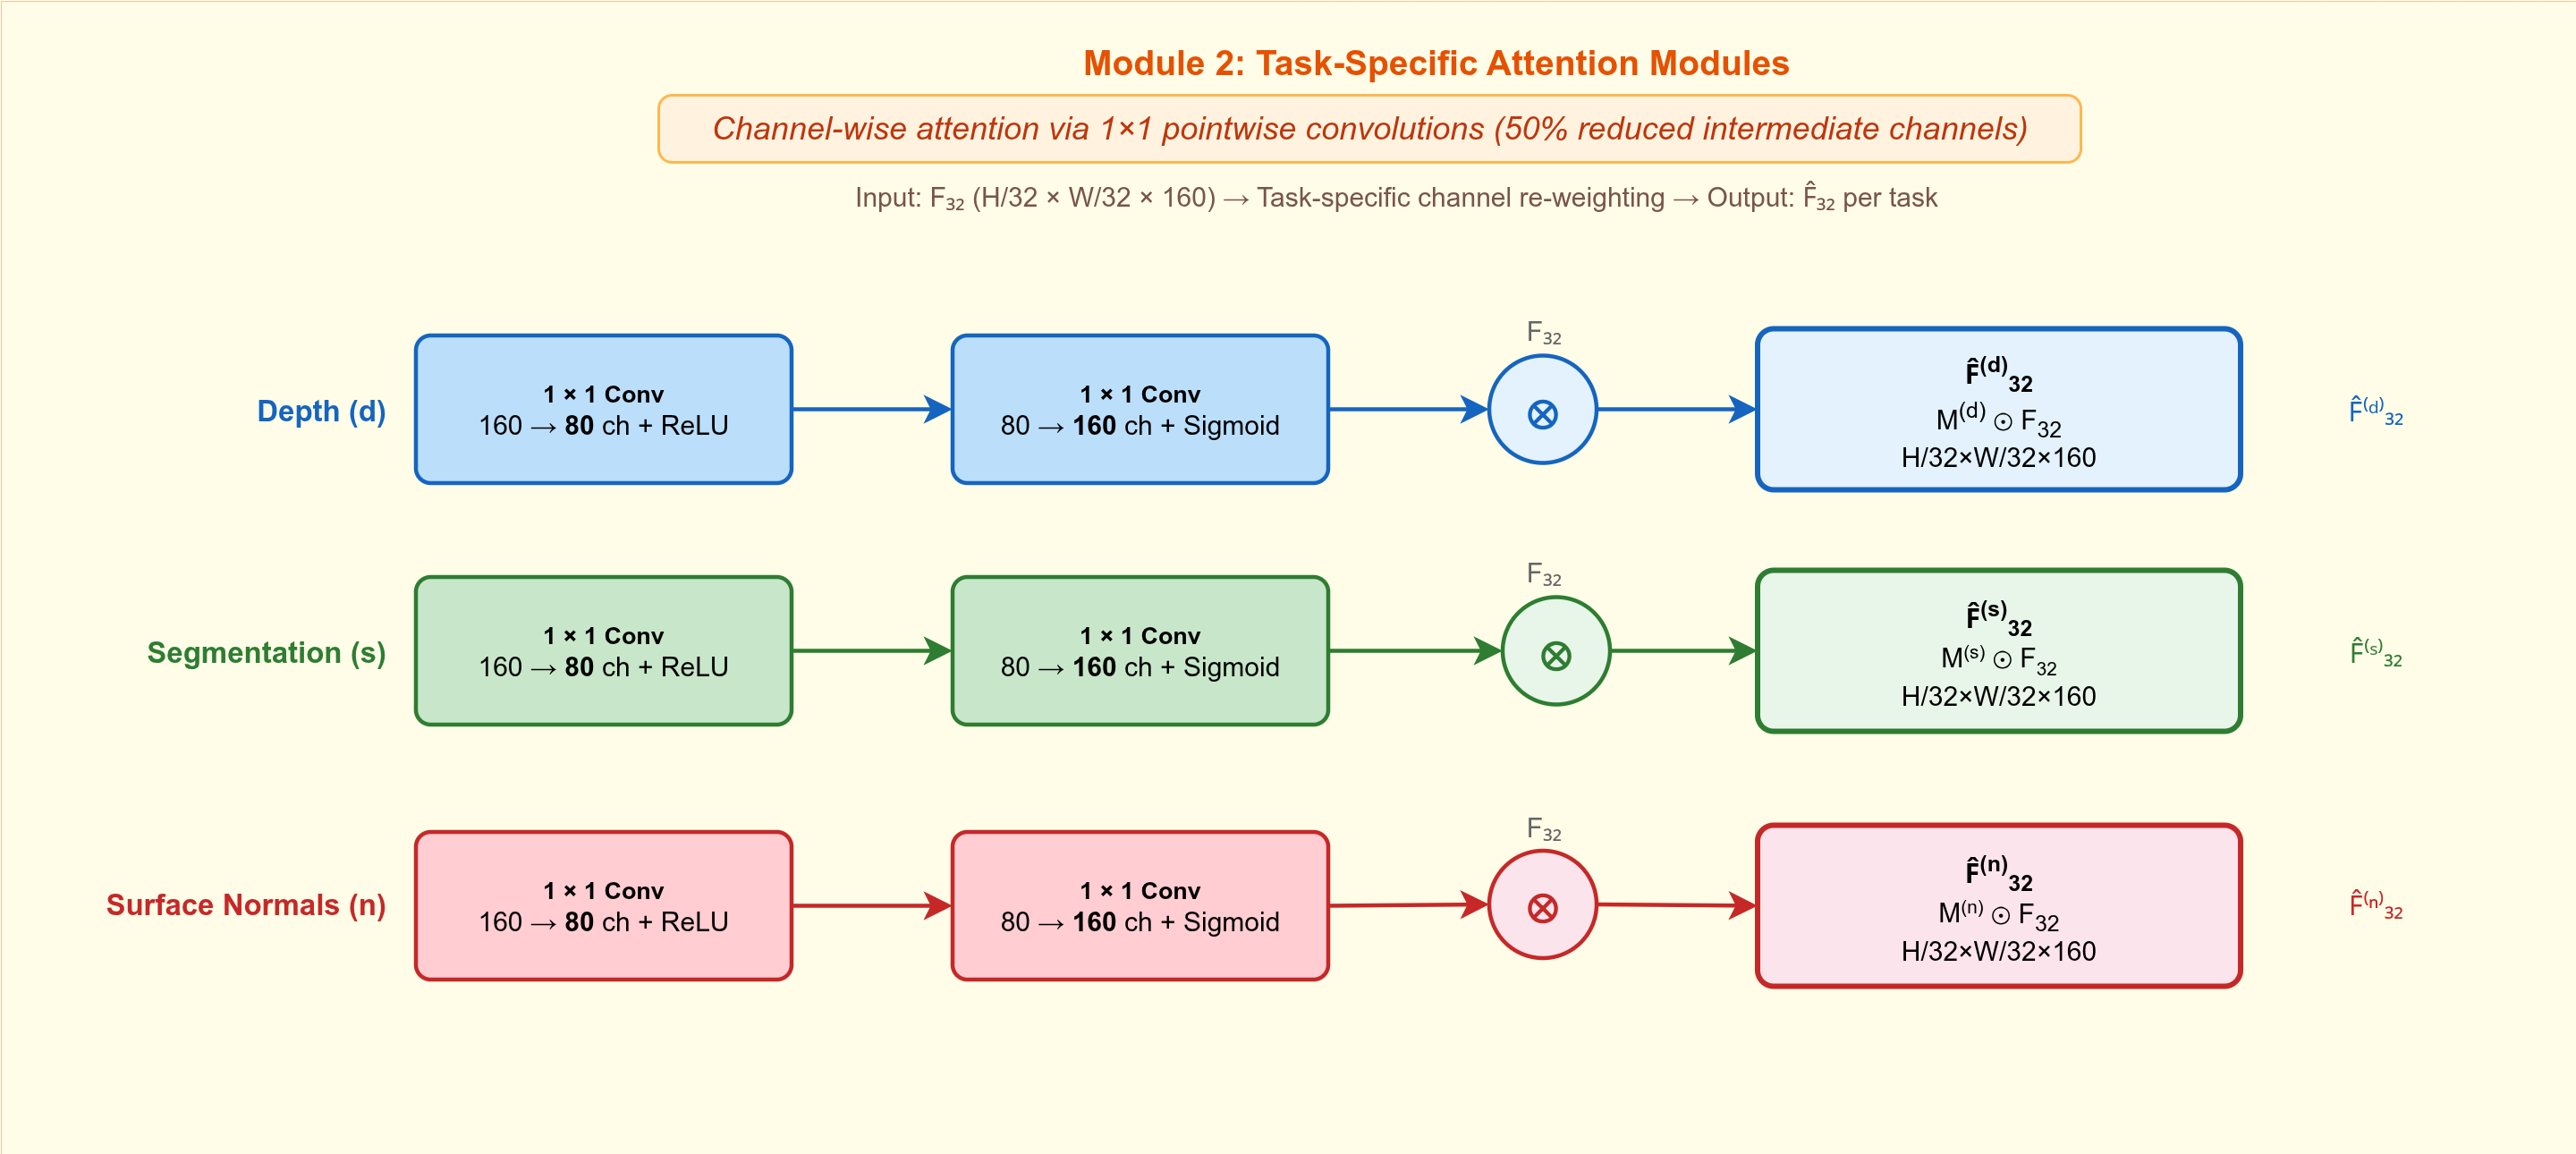
\includegraphics[width=\linewidth]{figures/arch_attention.png}
    \caption{Module 2: Task-specific attention with channel-wise bottleneck (160$\to$80$\to$160) and sigmoid gating.}
    \label{fig:arch_attention}
\end{subfigure}

\vspace{2pt}

% --- Module 3: Decoder ---
\begin{subfigure}[b]{0.85\columnwidth}
    \centering
    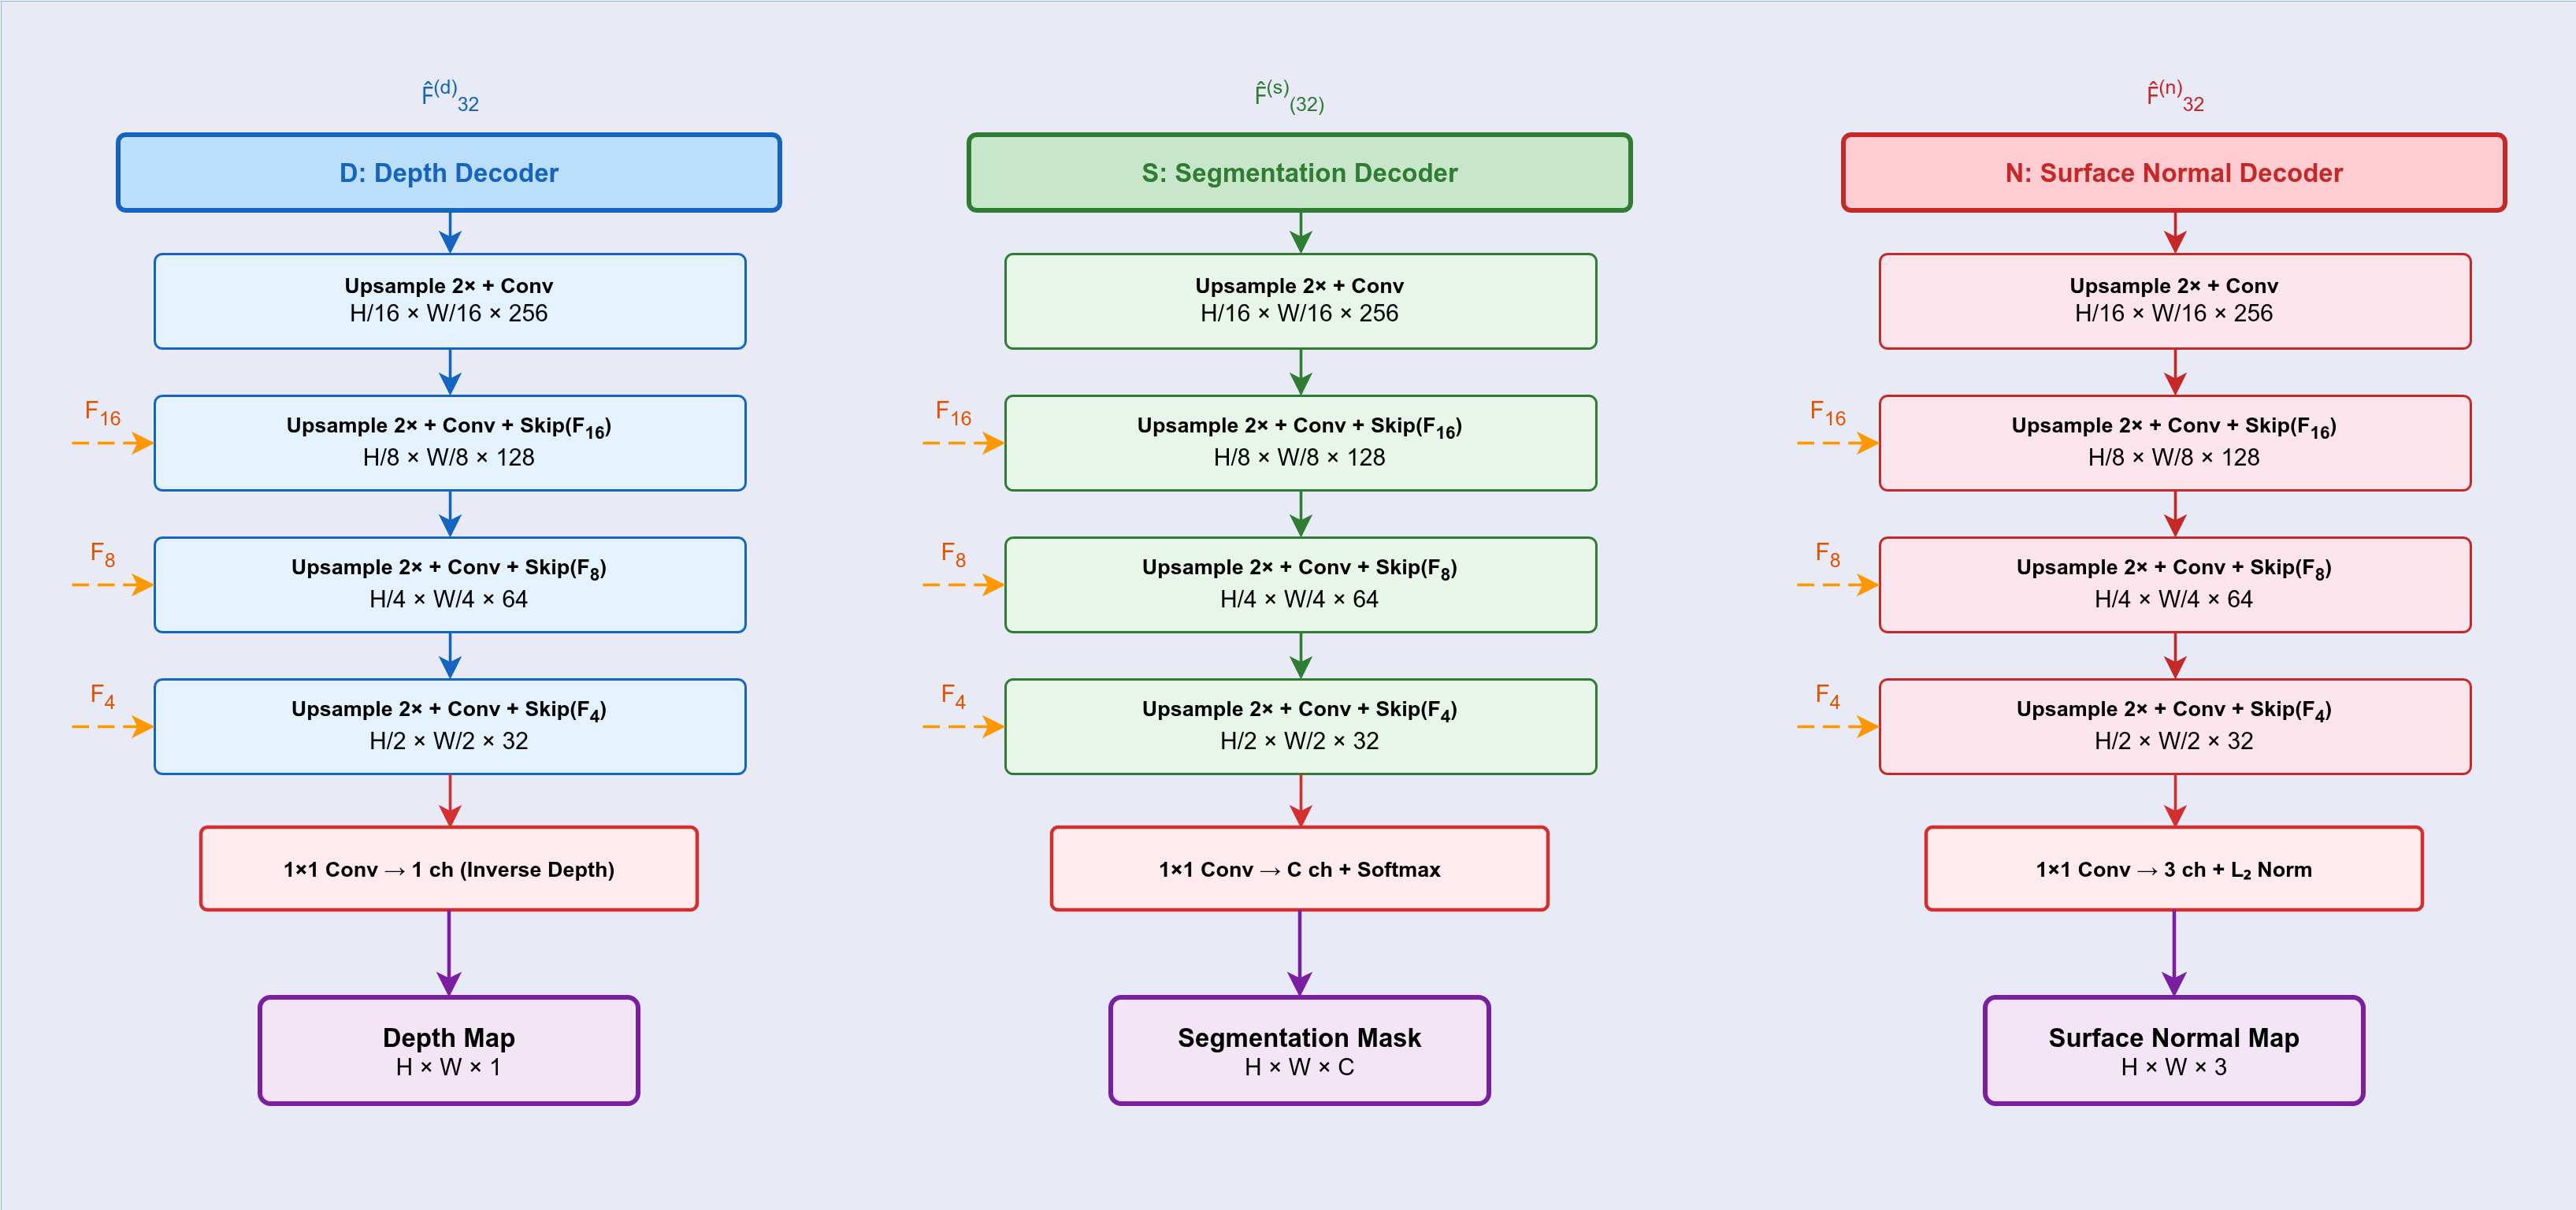
\includegraphics[width=\linewidth]{figures/arch_decoder.png}
    \caption{Module 3: Task-specific decoders with skip connections (256$\to$128$\to$64$\to$32).}
    \label{fig:arch_decoder}
\end{subfigure}

\caption{MTAN-Lite architecture. (a) Shared encoder extracts multi-scale features. (b) Attention modules selectively modulate features per task. (c) Parallel decoders reconstruct full-resolution predictions.}
\label{fig:architecture}
\end{figure}

\begin{table}[!htbp]
\centering
\caption{Parameter distribution of MTAN-Lite.}
\label{tab:params}
\renewcommand{\arraystretch}{1.2}
\begin{tabular}{lc}
\hline
\textbf{Component} & \textbf{Parameters} \\
\hline
MobileNetV3-Large encoder & 2.816M \\
Attention modules ($\times$3 tasks) & 0.078M \\
Depth decoder & 1.110M \\
Segmentation decoder & 1.110M \\
Surface normal decoder & 1.110M \\
\hline
\textbf{Total} & \textbf{6.224M} \\
\hline
\end{tabular}
\end{table}

\subsection{Shared Lightweight Encoder}

The shared encoder is a MobileNetV3-Large~\cite{howard2019mobilenetv3} backbone pretrained on ImageNet, selected for its favorable trade-off between representational capacity and computational cost. MobileNetV3 employs inverted residual blocks with depthwise separable convolutions, squeeze-and-excitation modules, and hard-swish activations, achieving strong classification accuracy at a fraction of the cost of conventional backbones such as ResNet-50 (25.6M parameters) or SegNet (29.4M parameters).

We extract intermediate features at four resolution scales by tapping into specific layers of the backbone:
\begin{equation}
\{F_4, F_8, F_{16}, F_{32}\} = \text{Enc}(I), \quad I \in \mathbb{R}^{H \times W \times 3}
\end{equation}
where $F_s \in \mathbb{R}^{H/s \times W/s \times C_s}$ denotes the feature map at stride $s$, with channel dimensions $C_4 = 24$, $C_8 = 40$, $C_{16} = 112$, and $C_{32} = 160$. The deepest feature map $F_{32}$ serves as input to the task-specific attention modules, while $F_4$, $F_8$, and $F_{16}$ are routed directly to the decoders as skip connections, providing fine-grained spatial detail at no additional computational cost since these features are already computed during the forward pass.

\subsection{Task-Specific Attention Modules}

Each task requires different subsets of the shared representation. Rather than learning entirely separate encoders so we introduced lightweight channel wise attention modules that allowed each task to selectively emphasize or suppress channels in $F_{32}$. For task $t \in \{d, s, n\}$ (depth, segmentation, normals) the attention mask is computed as:
\begin{equation}
M^{(t)} = \sigma\left(W_2^{(t)} \cdot \text{ReLU}\left(W_1^{(t)} \cdot F_{32}\right)\right)
\end{equation}
where $W_1^{(t)} \in \mathbb{R}^{80 \times 160}$ and $W_2^{(t)} \in \mathbb{R}^{160 \times 80}$ are pointwise ($1 \times 1$) convolution weights, and $\sigma$ denotes the sigmoid function. The bottleneck reduces the intermediate dimension from 160 to 80 channels (50\% reduction), decreasing attention module parameters by 75\% compared to a full-rank projection while still providing sufficient capacity for per-channel task relevance learning. Each attention module contributes only 0.026M parameters. The task-specific modulated features are obtained by element-wise multiplication:
\begin{equation}
\hat{F}_{32}^{(t)} = M^{(t)} \odot F_{32}
\end{equation}
This soft gating mechanism allows each task to amplify channels carrying task-relevant information while suppressing irrelevant activations, without altering the shared encoder weights.

\subsection{Task-Specific Decoders}

Each task has an independent decoder that progressively upsamples the attention modulated features $\hat{F}_{32}^{(t)}$ back to the input resolution through four stages. At each stage feature maps are bilinearly upsampled by $2\times$, concatenated with the corresponding encoder skip connection and projected to the target channel dimension through a convolutional block (Conv $3\times3$ + BatchNorm + ReLU). The stages produce feature maps with channel dimensions 256, 128, 64, and 32 at spatial resolutions $H/16$, $H/8$, $H/4$ and $H/2$ respectively. Skip connections from $F_{16}$, $F_8$ and $F_4$ inject multi-scale spatial details that would be otherwise lost through the attention bottleneck operating only on $F_{32}$. Each decoder contributes 1.110M parameters.

After the final decoder stage the task specific prediction heads produce the output for each task. The depth head uses a $1 \times 1$ convolution to a single channel with sigmoid activation, which produces an inverse depth map where higher values correspond to closer objects. The segmentation head projects to $C$ channels (19 for Cityscapes, 13 for NYUv2) with softmax activation for per pixel class probabilities. The surface normal head projects to 3 channels followed by L$_2$ normalization which applies the geometric constraint that normal vectors must lie on the same unit sphere.

\subsection{Multi-Task Loss Formulation}

The total training objective is a fixed weighted combination of three task specific losses which is
\begin{equation}
\mathcal{L}_{\text{total}} = \lambda_d \cdot \mathcal{L}_{\text{depth}} + \lambda_s \cdot \mathcal{L}_{\text{seg}} + \lambda_n \cdot \mathcal{L}_{\text{normal}}
\end{equation}
For Cityscapes, we used $\lambda_d = 1.0$, $\lambda_s = 4.0$, $\lambda_n = 0.5$ with the higher segmentation weight to compensate for smaller DiceFocal loss gradients and the lower normal weight reflecting in the noisier pseudo ground truths. For NYUv2, where all three tasks have sensor quality ground truths we use equal weights $\lambda_d = \lambda_s = \lambda_n = 1.0$.

\textbf{Depth loss.} We adopted the scale invariant loss from Eigen et al.~\cite{eigen2014depth}:
\begin{equation}
\mathcal{L}_{\text{depth}} = \frac{1}{N}\sum_i g_i^2 - \frac{0.5}{N^2}\left(\sum_i g_i\right)^2
\end{equation}
where $g_i = \log \hat{d}_i - \log d_i^{*}$ is the log-space residual between predicted and ground-truth depth at pixel $i$.

\textbf{Segmentation loss.} We combined the Dice loss with Focal loss~\cite{lin2017focal} in equal proportion ($\mathcal{L}_{\text{seg}} = 0.5 \cdot \mathcal{L}_{\text{Dice}} + 0.5 \cdot \mathcal{L}_{\text{Focal}}$). Dice loss optimizes per class overlap and treats each class equally regardless of pixel count. Focal loss with $\gamma = 2.0$ down weights confident predictions to focus learning on hard examples.

\textbf{Normal loss.} Since surface normals are unit vectors, their meaningful comparison is angular rather than Euclidean. We use cosine similarity loss ($1 - \hat{n}_i \cdot n_i^{*}$) averaged over valid pixels.

\subsection{Surface Normal Pseudo-Ground-Truth Generation}

The Cityscapes dataset does not provide native surface normal annotations. We generate pseudo-ground-truth normals from the available stereo disparity maps through a geometric pipeline that requires no learned components. For each frame, we convert stereo disparity $\delta$ to metric depth using per-frame camera parameters:
\begin{equation}
z(u,v) = \frac{b \cdot f_x}{\delta(u,v)}
\end{equation}
where $b$ is the stereo baseline and $f_x$ is the horizontal focal length. The depth map is then converted to surface normals using the DSINE~\cite{bae2024dsine} depth-to-normal utility with a $5 \times 5$ finite-difference cross-product kernel. NYUv2 provides true Kinect-derived surface normals directly, requiring no pseudo-ground-truth generation.

% === EXPERIMENTAL SETUP ===
\section{Experimental Setup}

\subsection{Datasets}

\textbf{Cityscapes}~\cite{Cordts2016Cityscapes} is a widely used outdoor driving dataset with 2975 training and 500 validation images at $1024\times2048$ resolution, labeled with 19 semantic classes. We get depth maps from stereo disparity (covering roughly 1 to 80m) and derive surface normals from that depth using geometric cross-products. All our experiments use $512\times1024$ as the input resolution.

\textbf{NYUv2}~\cite{silberman2012nyu} is the standard indoor dataset for multi task dense prediction with 795 training and 654 validation images at $288\times384$ resolution. It comes with 13 class segmentation labels with real Kinect depth and sensor derived surface normals. Since most of the methods we compare against report numbers on NYUv2 evaluating with this is important for a fair comparison.

\subsection{Training Configuration}

\textbf{Cityscapes.} We trained for 80 epochs with Adam, starting at a learning rate of $1 \times 10^{-4}$ with cosine annealing down to $1 \times 10^{-6}$. Batch size is 2 because of the 4 GB VRAM limit on our GPU. For augmentation we used random scale jittering (0.5$\times$ to 2.0$\times$), random crop, horizontal flip, color jitter and Gaussian blur. The encoder is initialized with ImageNet pretrained weights. The best checkpoint ended up being at epoch 72. The whole training took around 48 hours on the GTX 1650.

\textbf{NYUv2.} We trained for 200 epochs using the same optimizer and augmentation setup. Batch size is 4 and we use equal loss weights ($\lambda_d = \lambda_s = \lambda_n = 1.0$). The only architectural change was that the segmentation head outputs 13 classes instead of 19; everything else stays the same. Best checkpoint was at epoch 156 and training takes about 2.2 hours on the same GPU.

\subsection{Evaluation Metrics}

\textbf{Semantic segmentation}: we compute mIoU across all validation images.

\textbf{Monocular depth}: we compute threshold accuracy $\delta_1$ ($\max(\hat{d}/d^{*}, d^{*}/\hat{d}) < 1.25$), absolute relative error (AbsRel) and RMSE.

\textbf{Surface normals}: we compute mean angular error (MAE), median angular error (MedAE) and weighted angular error (WAE).

\textbf{Inference efficiency}: we also report frames per second (FPS) and peak GPU memory on GTX 1650.

\subsection{Baselines}

For Cityscapes, we compared against MTAN~\cite{liu2019mtan}, DenseMTL~\cite{lopes2023densemtl}, PAD-Net~\cite{xu2018padnet}, LAKNet~\cite{laknet2025}, SegFormer-B0~\cite{xie2021segformer}, and DeepLabv3+ MobileNetV2~\cite{chen2018deeplabv3plus}. For NYUv2, we compared against MTAN, PAD-Net, MTI-Net~\cite{vandenhende2020mti}, InvPT~\cite{ye2022invpt} and MTMamba~\cite{lin2024mtmamba}. All baseline numbers are from their respective publications.

% === RESULTS ===
\section{Results and Analysis}

\subsection{MTAN-Lite Results on Cityscapes}

Table~\ref{tab:cityscapes_results} presents the complete evaluation of MTAN-Lite on the Cityscapes validation set on all three tasks along with efficiency metrics.

\begin{table}[!htbp]
\centering
\caption{MTAN-Lite detailed results on the Cityscapes validation set (19-class, $512\times1024$ resolution).}
\label{tab:cityscapes_results}
\renewcommand{\arraystretch}{1.2}
\begin{tabular}{llc}
\hline
\textbf{Task} & \textbf{Metric} & \textbf{Value} \\
\hline
\multirow{3}{*}{Segmentation} & mIoU (19-class) & 70.1\% \\
 & Best class (road) & 97.2\% \\
 & Worst class (wall) & 49.0\% \\
\hline
\multirow{3}{*}{Depth} & $\delta_1$ ($<$1.25) & 0.849 \\
 & AbsRel & 0.123 \\
 & RMSE & 7.50\,m \\
\hline
\multirow{2}{*}{Normals} & MAE & 49.1$^\circ$ \\
 & WAE & 48.5$^\circ$ \\
\hline
\multirow{4}{*}{Efficiency} & Parameters & 6.2M \\
 & FPS (GTX 1650) & 39.6 \\
 & Latency & 25.2\,ms \\
 & GPU Memory & 102\,MB \\
\hline
\end{tabular}
\end{table}

MTAN-Lite gets 70.1\% mIoU on 19 class Cityscapes. This is only 1.8\% below SegFormer-B0~\cite{xie2021segformer} (71.9\%, 3.8M parameters) and 2.4\% below DeepLabv3+ MobileNetV2~\cite{chen2018deeplabv3plus} (72.5\%, 5.8M parameters) but those are segmentation only models. Our model also predicts depth (84.9\% $\delta_1$) and surface normals (49.1$^\circ$ MAE) alongside segmentation so the small gap seems like a fair trade-off. When compared with MTAN~\cite{liu2019mtan}, which uses a SegNet backbone with 32.4M parameters and was only tested with 7 classes at 128$\times$256 without normals our model has 81\% fewer parameters, handles 16$\times$ more pixels, does an extra task and uses all 19 classes. LAKNet~\cite{laknet2025} has 38.6M parameters which is 6.2$\times$ larger than ours and only does segmentation and depth without normals. DenseMTL~\cite{lopes2023densemtl} does include normals on Cityscapes with HRNet-18, but they only use 16 classes and do not report inference speed. As far only our work is the first to do three task prediction on the full 19-class Cityscapes with a lightweight model at real time speed.

\FloatBarrier
\subsection{Cross-Dataset Evaluation on NYUv2}

We also wanted to check if our MTAN Lite works beyond outdoor driving scenes so we tested it on NYUv2~\cite{silberman2012nyu} which is the go to indoor benchmark for multi-task methods. Table~\ref{tab:nyuv2_results} shows our numbers alongside published results from other methods.

\begin{table}[!htbp]
\centering
\caption{Comparison on NYUv2 validation set (13-class segmentation, depth, surface normals). All methods use $288 \times 384$ resolution. Best lightweight ($<$10M) result in \textbf{bold}.}
\label{tab:nyuv2_results}
\renewcommand{\arraystretch}{1.2}
\begin{tabular}{lccccc}
\hline
\textbf{Method} & \textbf{Backbone} & \textbf{Params} & \textbf{mIoU$\uparrow$} & \textbf{RMSE$\downarrow$} & \textbf{N-mErr$\downarrow$} \\
\hline
MTAN & SegNet & 32.4M & $\sim$22 & 0.631 & 27.8$^\circ$ \\
PAD-Net & ResNet-50 & $>$25M & 36.6 & 0.582 & 20.9$^\circ$ \\
MTI-Net & HRNet-18 & $>$20M & 46.0 & 0.536 & 20.3$^\circ$ \\
InvPT & ViT-Large & $>$300M & 53.6 & 0.518 & 19.0$^\circ$ \\
MTMamba & Swin-Large & $>$100M & 55.8 & 0.507 & 18.6$^\circ$ \\
\hline
\textbf{Ours} & \textbf{MNV3-L} & \textbf{6.2M} & \textbf{51.7} & \textbf{0.621} & \textbf{23.9$^\circ$} \\
\hline
\end{tabular}
\end{table}

On NYUv2, MTAN-Lite reaches 51.7\% mIoU, which is well above MTAN ($\sim$22\%), PAD-Net (36.6\%), and MTI-Net (46.0\%), all of which use 3 to 5$\times$ more parameters. Depth RMSE comes out to 0.621m, close to MTAN's 0.631m, and the normal MAE of 23.9$^\circ$ is much better than MTAN's 27.8$^\circ$. A big reason for the improved normals is that NYUv2 has real sensor ground truth instead of the noisy pseudo-labels we use on Cityscapes. InvPT and MTMamba do get higher mIoU (53.6\% and 55.8\%), but they need 50 to 100$\times$ more parameters. As far as we are aware, MTAN-Lite is the only model under 10M parameters doing all three tasks on NYUv2.

\FloatBarrier
\subsection{Per-Class Segmentation Analysis}

\begin{figure}[!htbp]
\centering
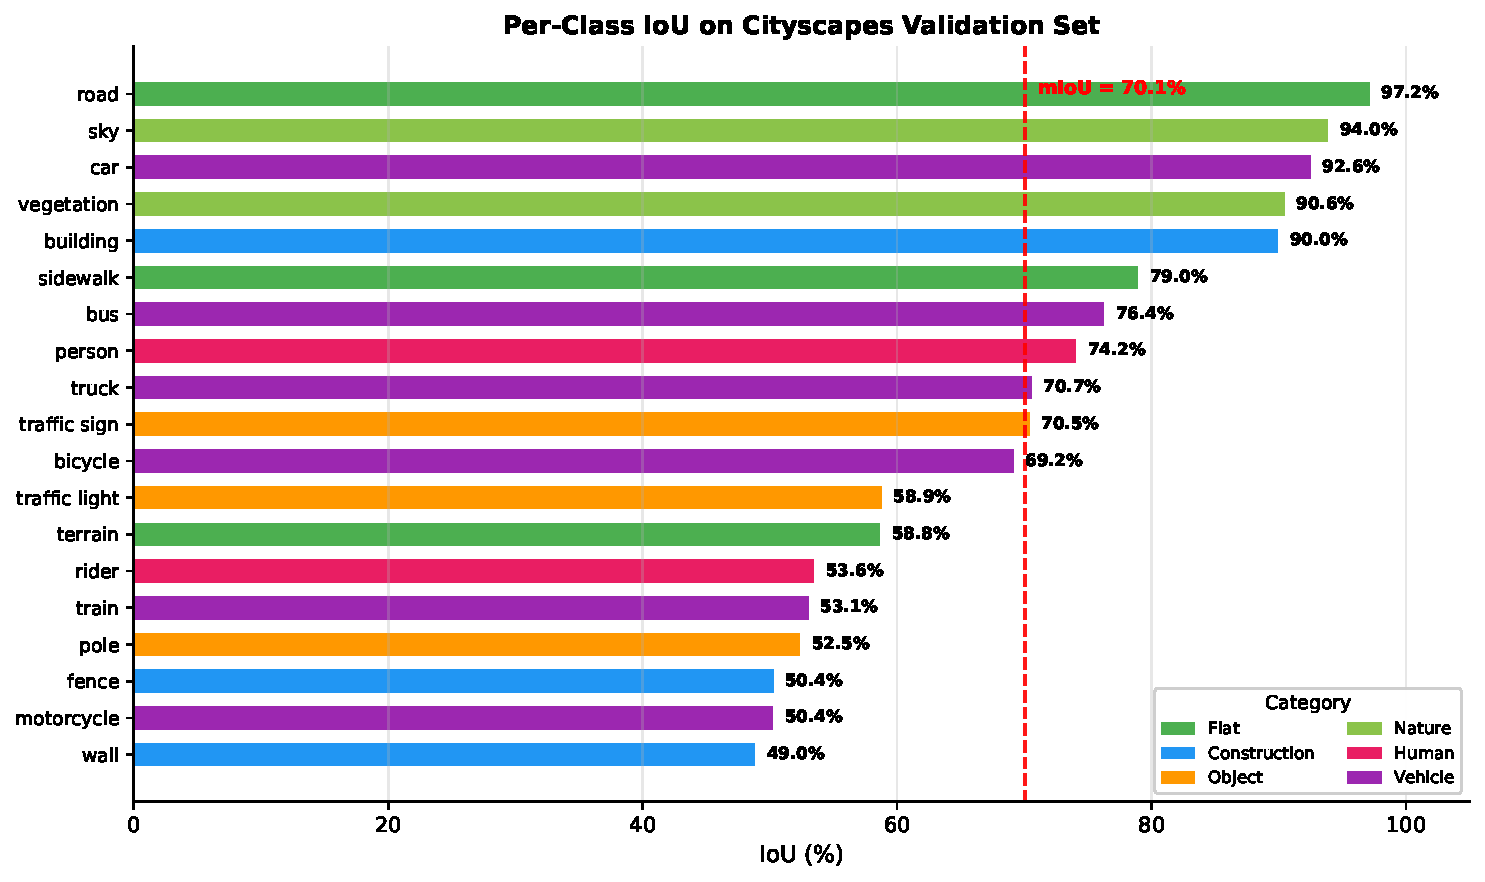
\includegraphics[width=\columnwidth]{figures/per_class_iou.pdf}
\caption{Per-class IoU on the Cityscapes validation set. All 19 classes exceed 48\% IoU. Dominant spatial classes (road, building, vegetation, sky, car) exceed 90\%, while geometrically small or rare classes (wall, fence, motorcycle) cluster near 50\%.}
\label{fig:per_class_iou}
\end{figure}

\begin{figure}[!htbp]
\centering
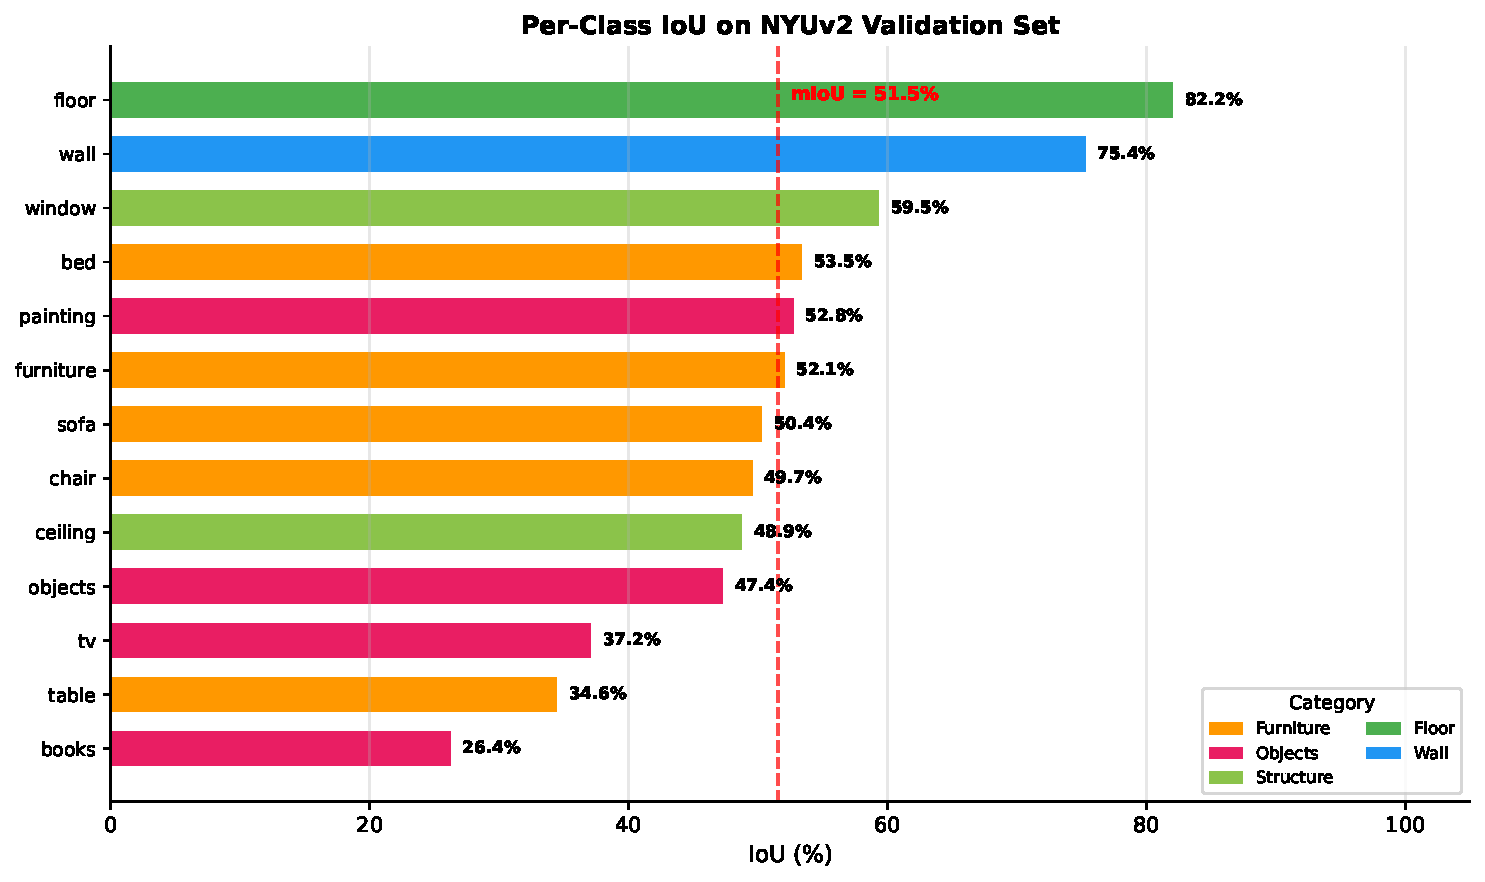
\includegraphics[width=\columnwidth]{eval_results/nyuv2/per_class_iou.pdf}
\caption{Per-class IoU on the NYUv2 validation set. All 13 indoor classes are represented. Dominant planar classes (floor, wall, ceiling) achieve the highest IoU, while small or geometrically complex classes (books, tv, painting) present greater challenge.}
\label{fig:per_class_iou_nyuv2}
\end{figure}

Fig.~\ref{fig:per_class_iou} shows the per-class IoU for Cityscapes. The large spatial classes do well as expected: road gets 97.2\%, sky 94.0\%, car 92.6\%, vegetation 90.6\%, and building 90.1\%. The harder classes are wall (49.0\%), fence (50.4\%), and motorcycle (50.4\%), which is not surprising given how small they are in the image and how similar they look to neighboring classes. The important thing is that no class drops below 48\%, which tells us that the DiceFocal loss is doing its job and model is not just ignoring rare categories.

Fig.~\ref{fig:per_class_iou_nyuv2} has the NYUv2 per-class results. Indoor scenes have a different set of challenges, like large flat surfaces like floors, walls and ceilings are segmented well but smaller objects like books, tv, painting and classes with lots of intra class variation like furniture, objects are harder to get right. Even then the model is able to get above 40\% IoU on all classes which is a good sign that the multi-task learning is helping the model learn better features for segmentation even with the less parameters

\FloatBarrier
\subsection{Surface Normal Analysis}

\begin{figure}[!htbp]
\centering

\includegraphics[width=\columnwidth]{eval_results/radar_sne_metrics.png}
\caption{Per category surface normal metrics on Cityscapes. (a) Mean Angular Error and (b) Weighted Angular Error. Larger area = lower error = better. Flat surfaces (roadway, walkway) show the lowest error, complex geometry presents greater challenge due to noisy pseudo ground truths.}
\label{fig:radar_normals}
\end{figure}

\begin{figure}[!htbp]
\centering
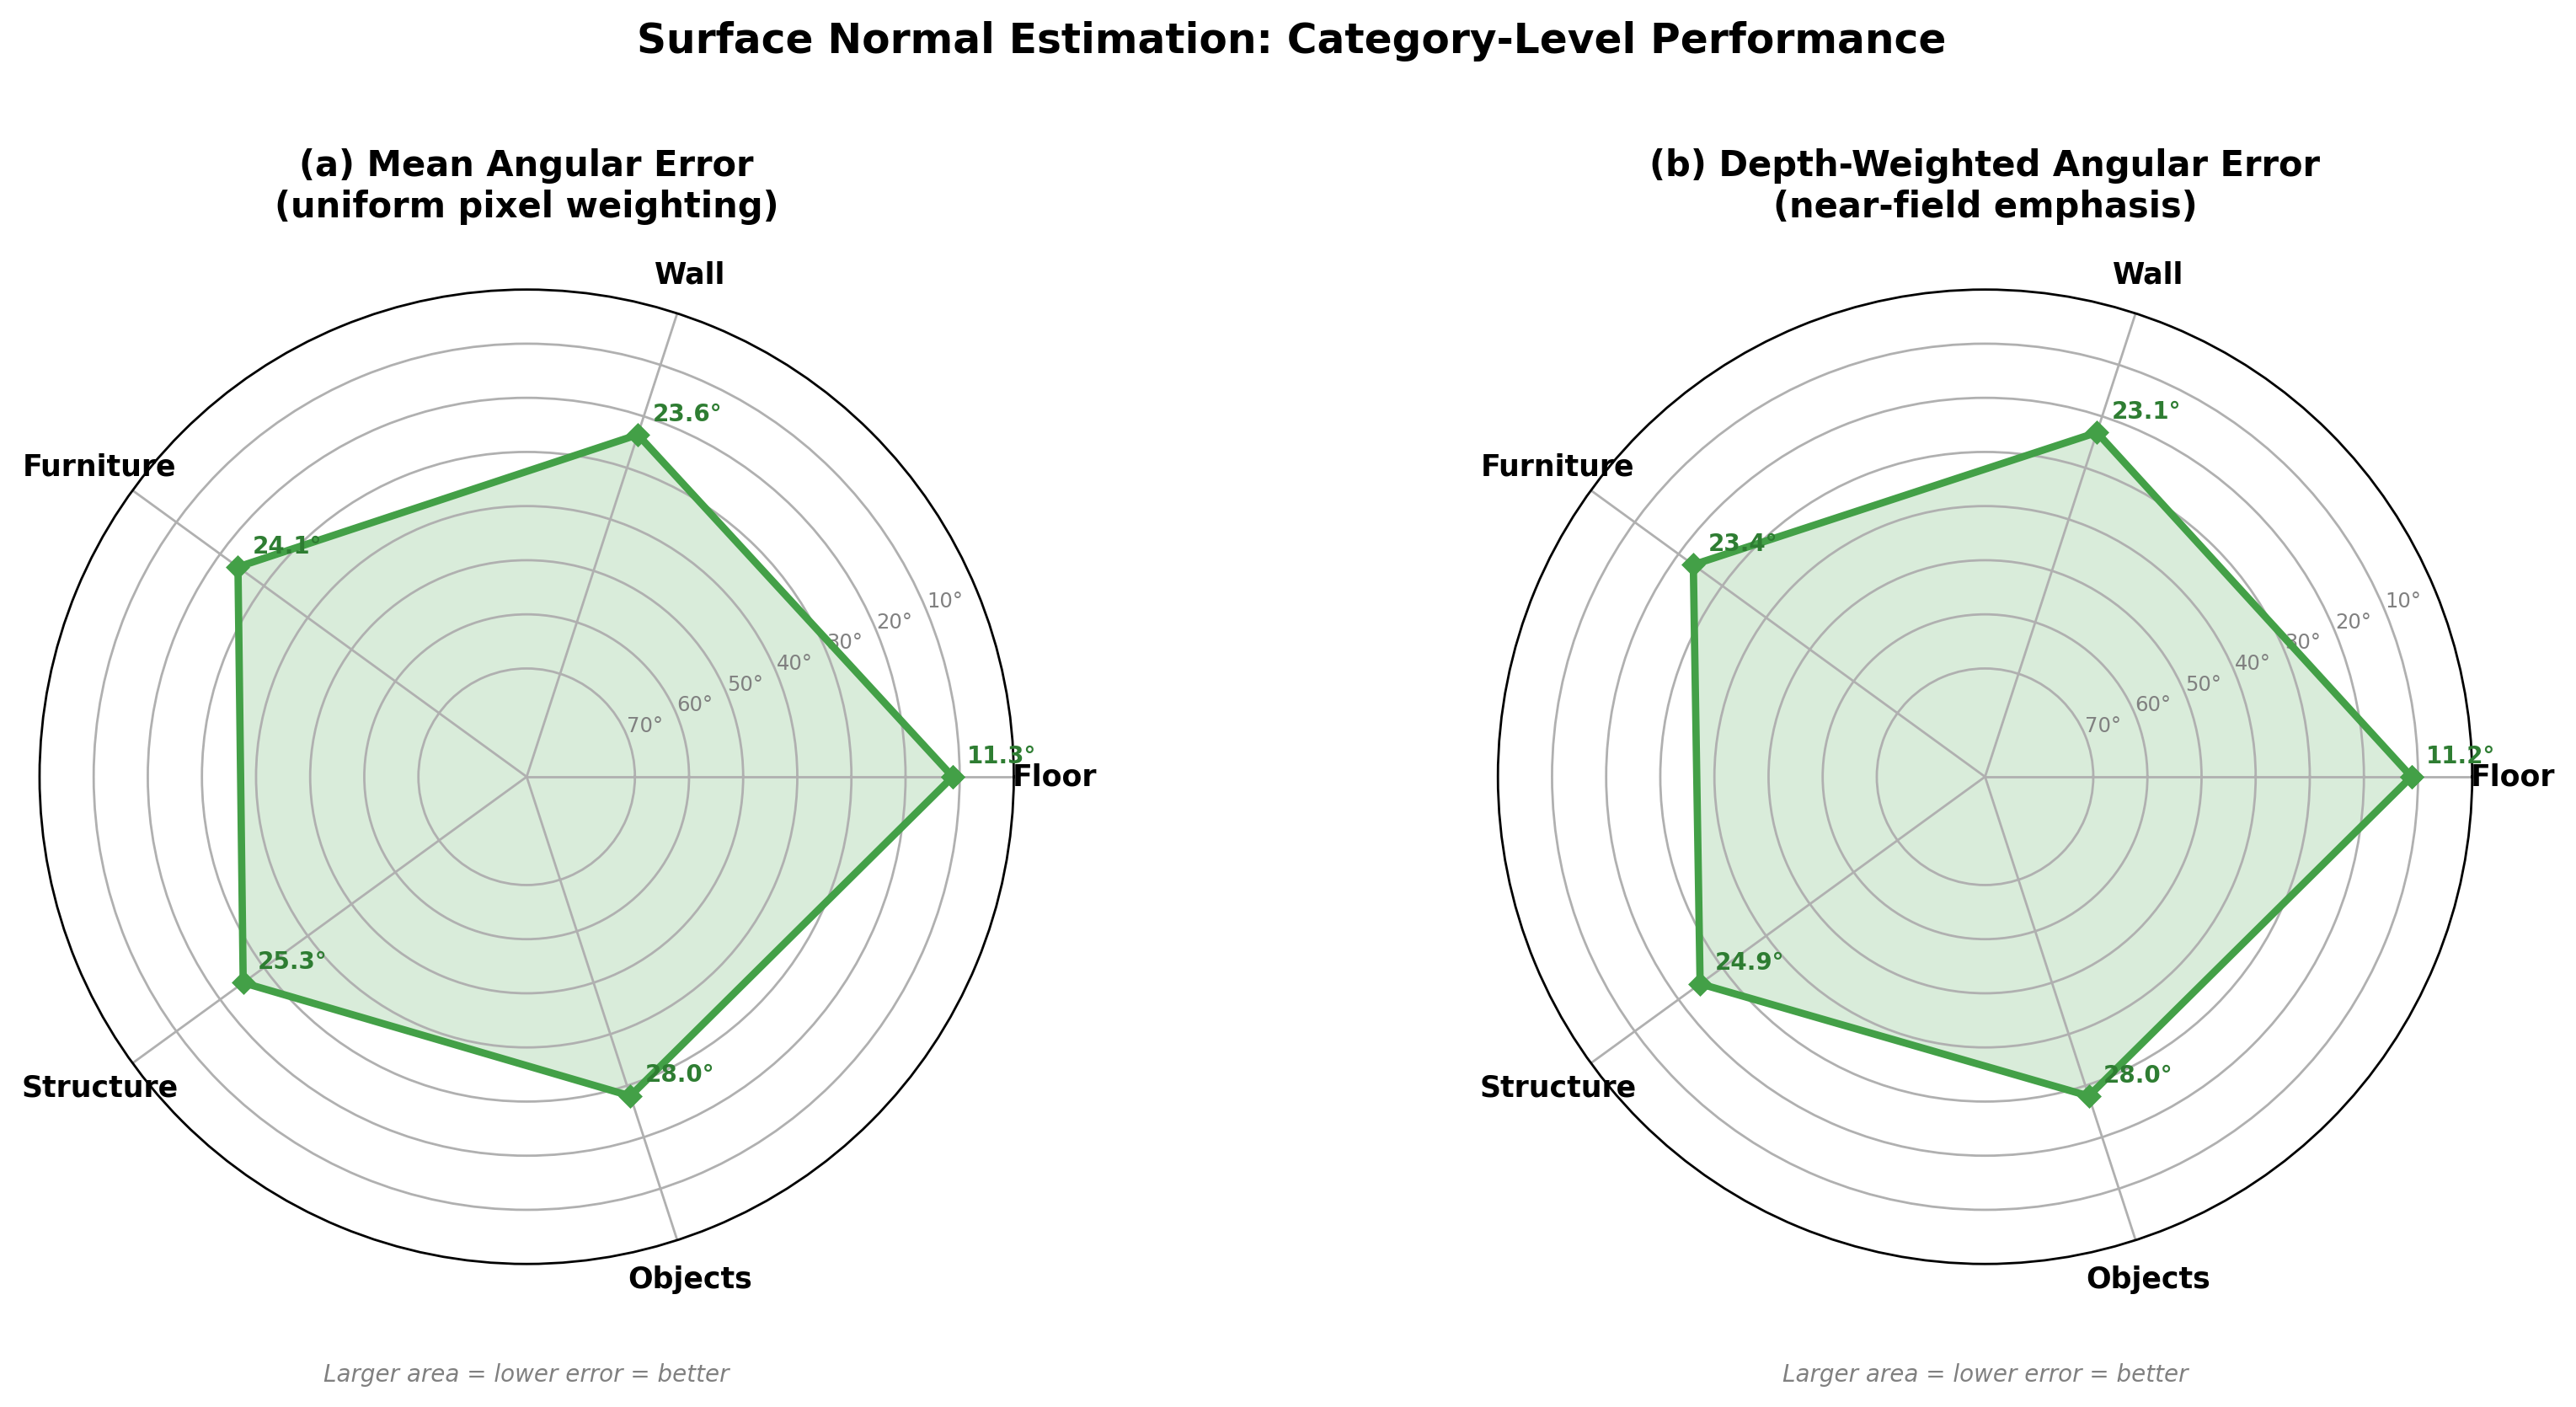
\includegraphics[width=\columnwidth]{eval_results/nyuv2/radar_sne_metrics.png}
\caption{Per-category surface normal metrics on NYUv2. (a) Mean Angular Error and (b) Weighted Angular Error. Indoor categories benefit from true sensor normals, with floor and wall surfaces achieving the lowest errors. The overall MAE of 23.9$^\circ$ (vs 49.1$^\circ$ on Cityscapes) confirms that sensor ground truth enables significantly better normal supervision.}
\label{fig:radar_normals_nyuv2}
\end{figure}

Fig.~\ref{fig:radar_normals} breaks down Cityscapes normal prediction by category. Flat surfaces like roadway and walkway has the lowest errors (MAE of 25.1$^\circ$ and 32.7$^\circ$) which makes sense since these are mostly planar and the stereo derived pseudo ground truths which is most reliable there. Building and vegetation are much worse (MAE around 70$^\circ$), partly because of the complex geometry but also because the pseudo ground truths itself is noisy at depth discontinuities.

Fig.~\ref{fig:radar_normals_nyuv2} shows the same analysis on NYUv2. The indoor categories benefit from having real Kinect derived normals and floor and wall surfaces get the lowest errors. The fact that overall MAE drops from 49.1$^\circ$ on Cityscapes to 23.9$^\circ$ on NYUv2 is a strong indication that pseudo ground truth quality not network capacity is what limits normal prediction on Cityscapes.

\FloatBarrier
\subsection{Ablation Study: Multi-Task vs Single-Task}

\begin{table}[!htbp]
\centering
\caption{Ablation study on Cityscapes comparing multi-task (full model) against single-task variants. Best results per metric in \textbf{bold}.}
\label{tab:ablation}
\renewcommand{\arraystretch}{1.2}
\begin{tabular}{lcccc}
\hline
\textbf{Variant} & \textbf{mIoU (\%)} & $\boldsymbol{\delta_1}$ & \textbf{AbsRel} & \textbf{N-MAE (\textdegree)} \\
\hline
Depth only & -- & \textbf{0.855} & \textbf{0.118} & -- \\
Seg only & 66.8 & -- & -- & -- \\
Normal only & -- & -- & -- & \textbf{48.6} \\
\hline
\textbf{MTAN-Lite (3 tasks)} & \textbf{70.1} & 0.849 & 0.123 & 49.1 \\
\hline
\end{tabular}
\end{table}

Table~\ref{tab:ablation} compares the full multi task model against single-task variants. The most notable result is that multi-task learning actually helps segmentation where mIoU goes up by 3.3\% (from 66.8\% to 70.1\%) compared to training segmentation alone. Depth $\delta_1$ only drops 0.6\% and normal MAE goes up by just 0.5$^\circ$ so the attention mechanism seems to be doing a good job of keeping the tasks from hurting each other.

\FloatBarrier
\subsection{Inference Efficiency}

MTAN-Lite runs at 39.6 FPS (about 25.2 ms per frame) on an NVIDIA GTX 1650 with 512$\times$1024 input, which is comfortably above the 30 FPS threshold which typically considered real time. Peak GPU memory usage is 102 MB. At 6.2M parameters, the model is 5.2$\times$ smaller than MTAN (32.4M) and much smaller than InvPT or MTMamba.

\FloatBarrier
\subsection{Qualitative Results}

\begin{figure}[!htbp]
\centering
\setlength{\tabcolsep}{2pt}
\begin{tabular}{cc}

\includegraphics[width=0.48\columnwidth]{eval_results/visualisations/sample_0000.png} &

\includegraphics[width=0.48\columnwidth]{eval_results/visualisations/sample_0001.png} \\[2pt]

\includegraphics[width=0.48\columnwidth]{eval_results/visualisations/sample_0002.png} &

\includegraphics[width=0.48\columnwidth]{eval_results/visualisations/sample_0003.png} \\
\end{tabular}
\caption{Qualitative predictions on Cityscapes validation images. Each panel shows (top row) input RGB, predicted depth, predicted segmentation, and predicted surface normals; (bottom row) corresponding ground truth.}
\label{fig:qualitative}
\end{figure}

\begin{figure}[!htbp]
\centering
\setlength{\tabcolsep}{2pt}
\begin{tabular}{cc}
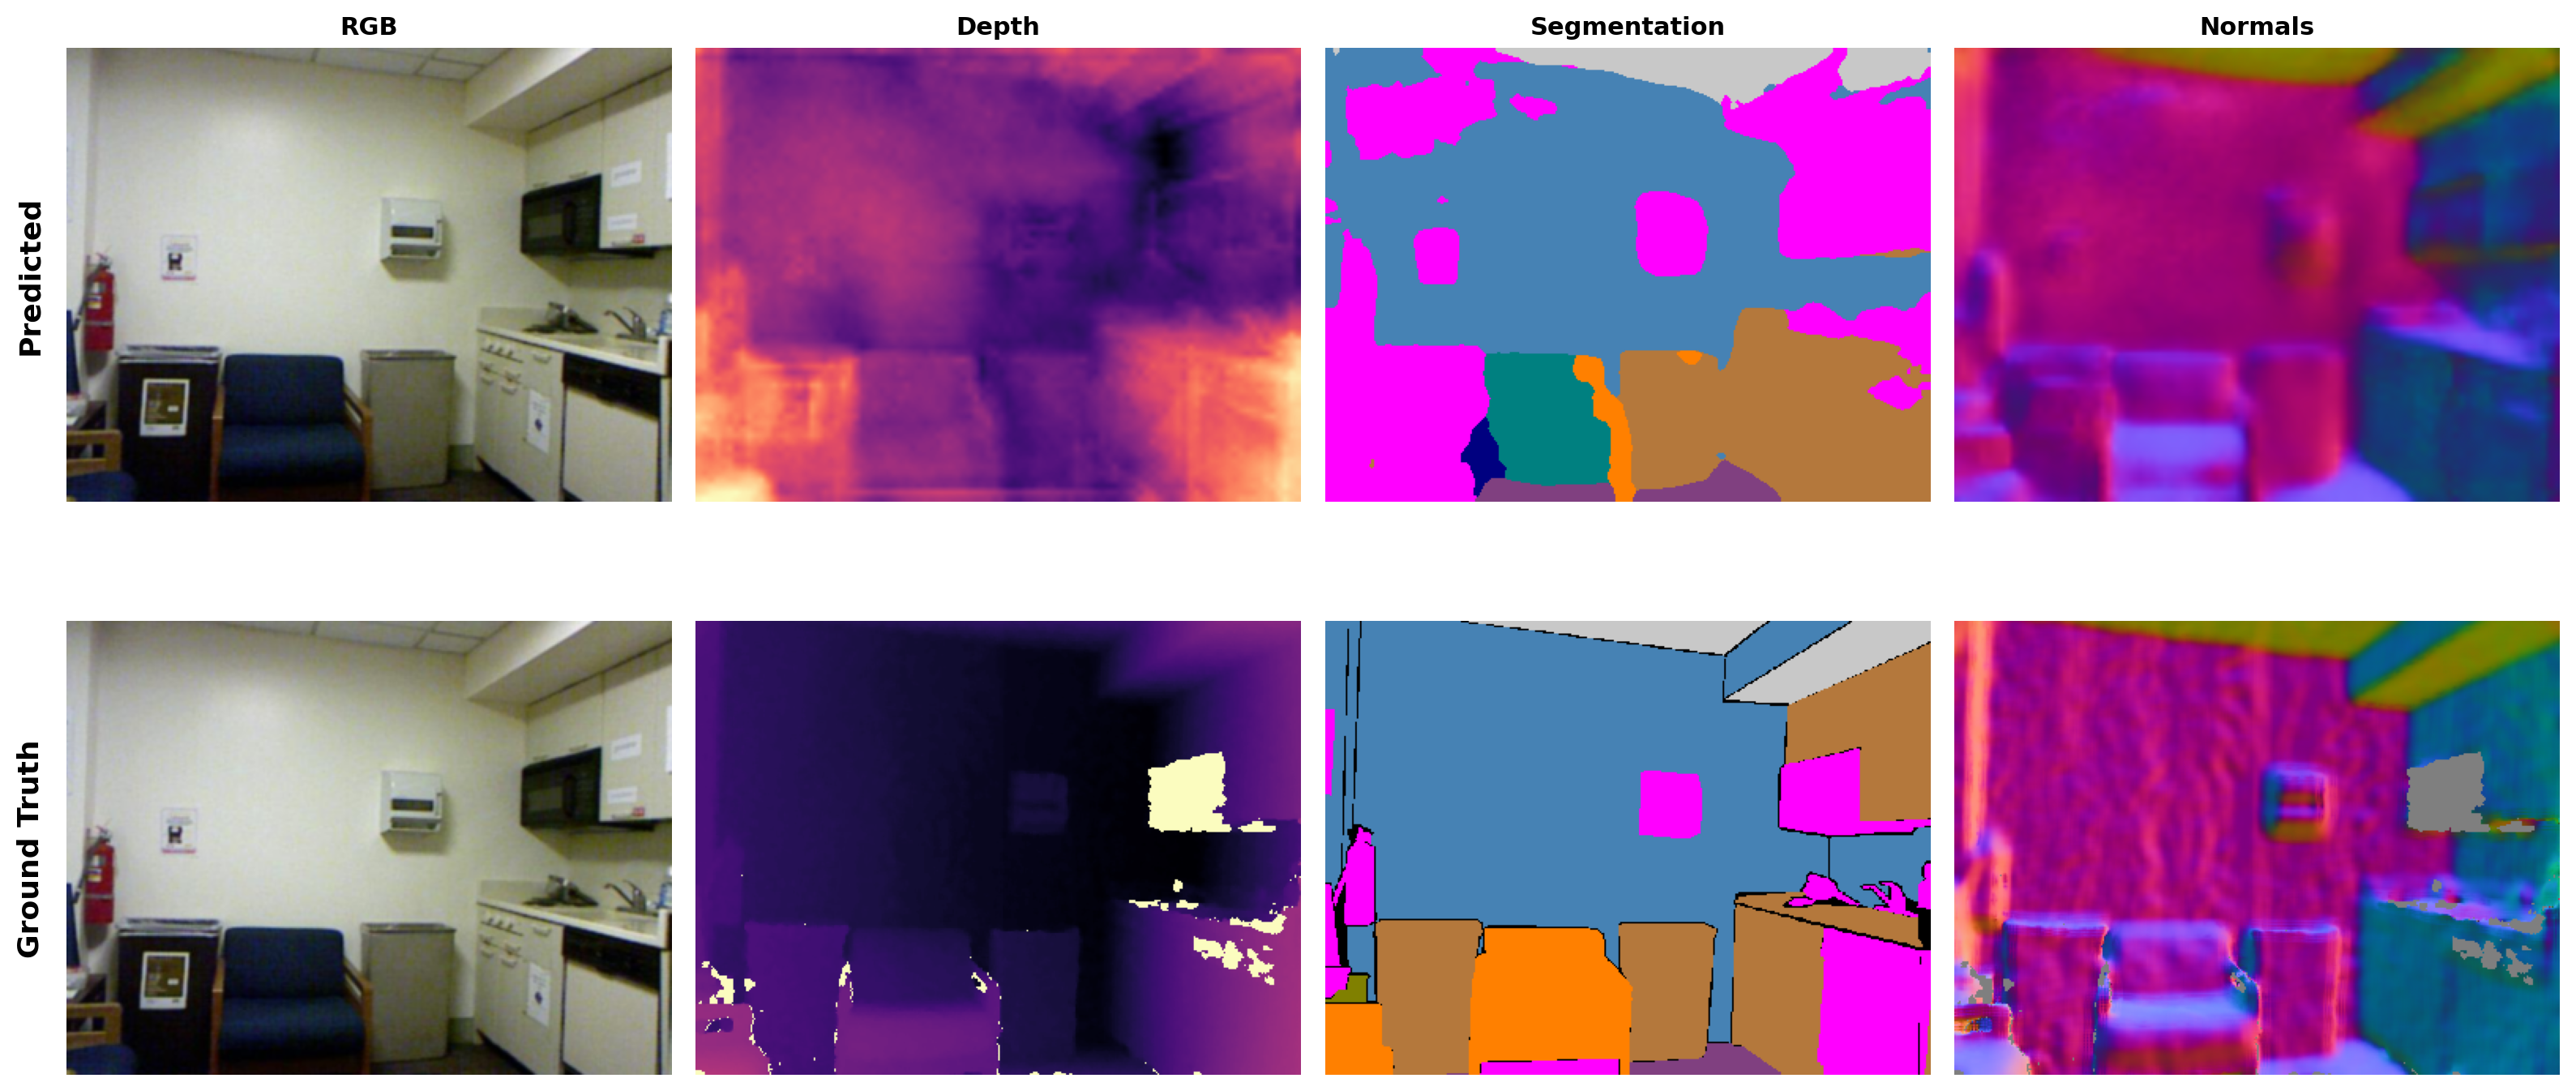
\includegraphics[width=0.48\columnwidth]{eval_results/nyuv2/visualisations/sample_0000.png} &
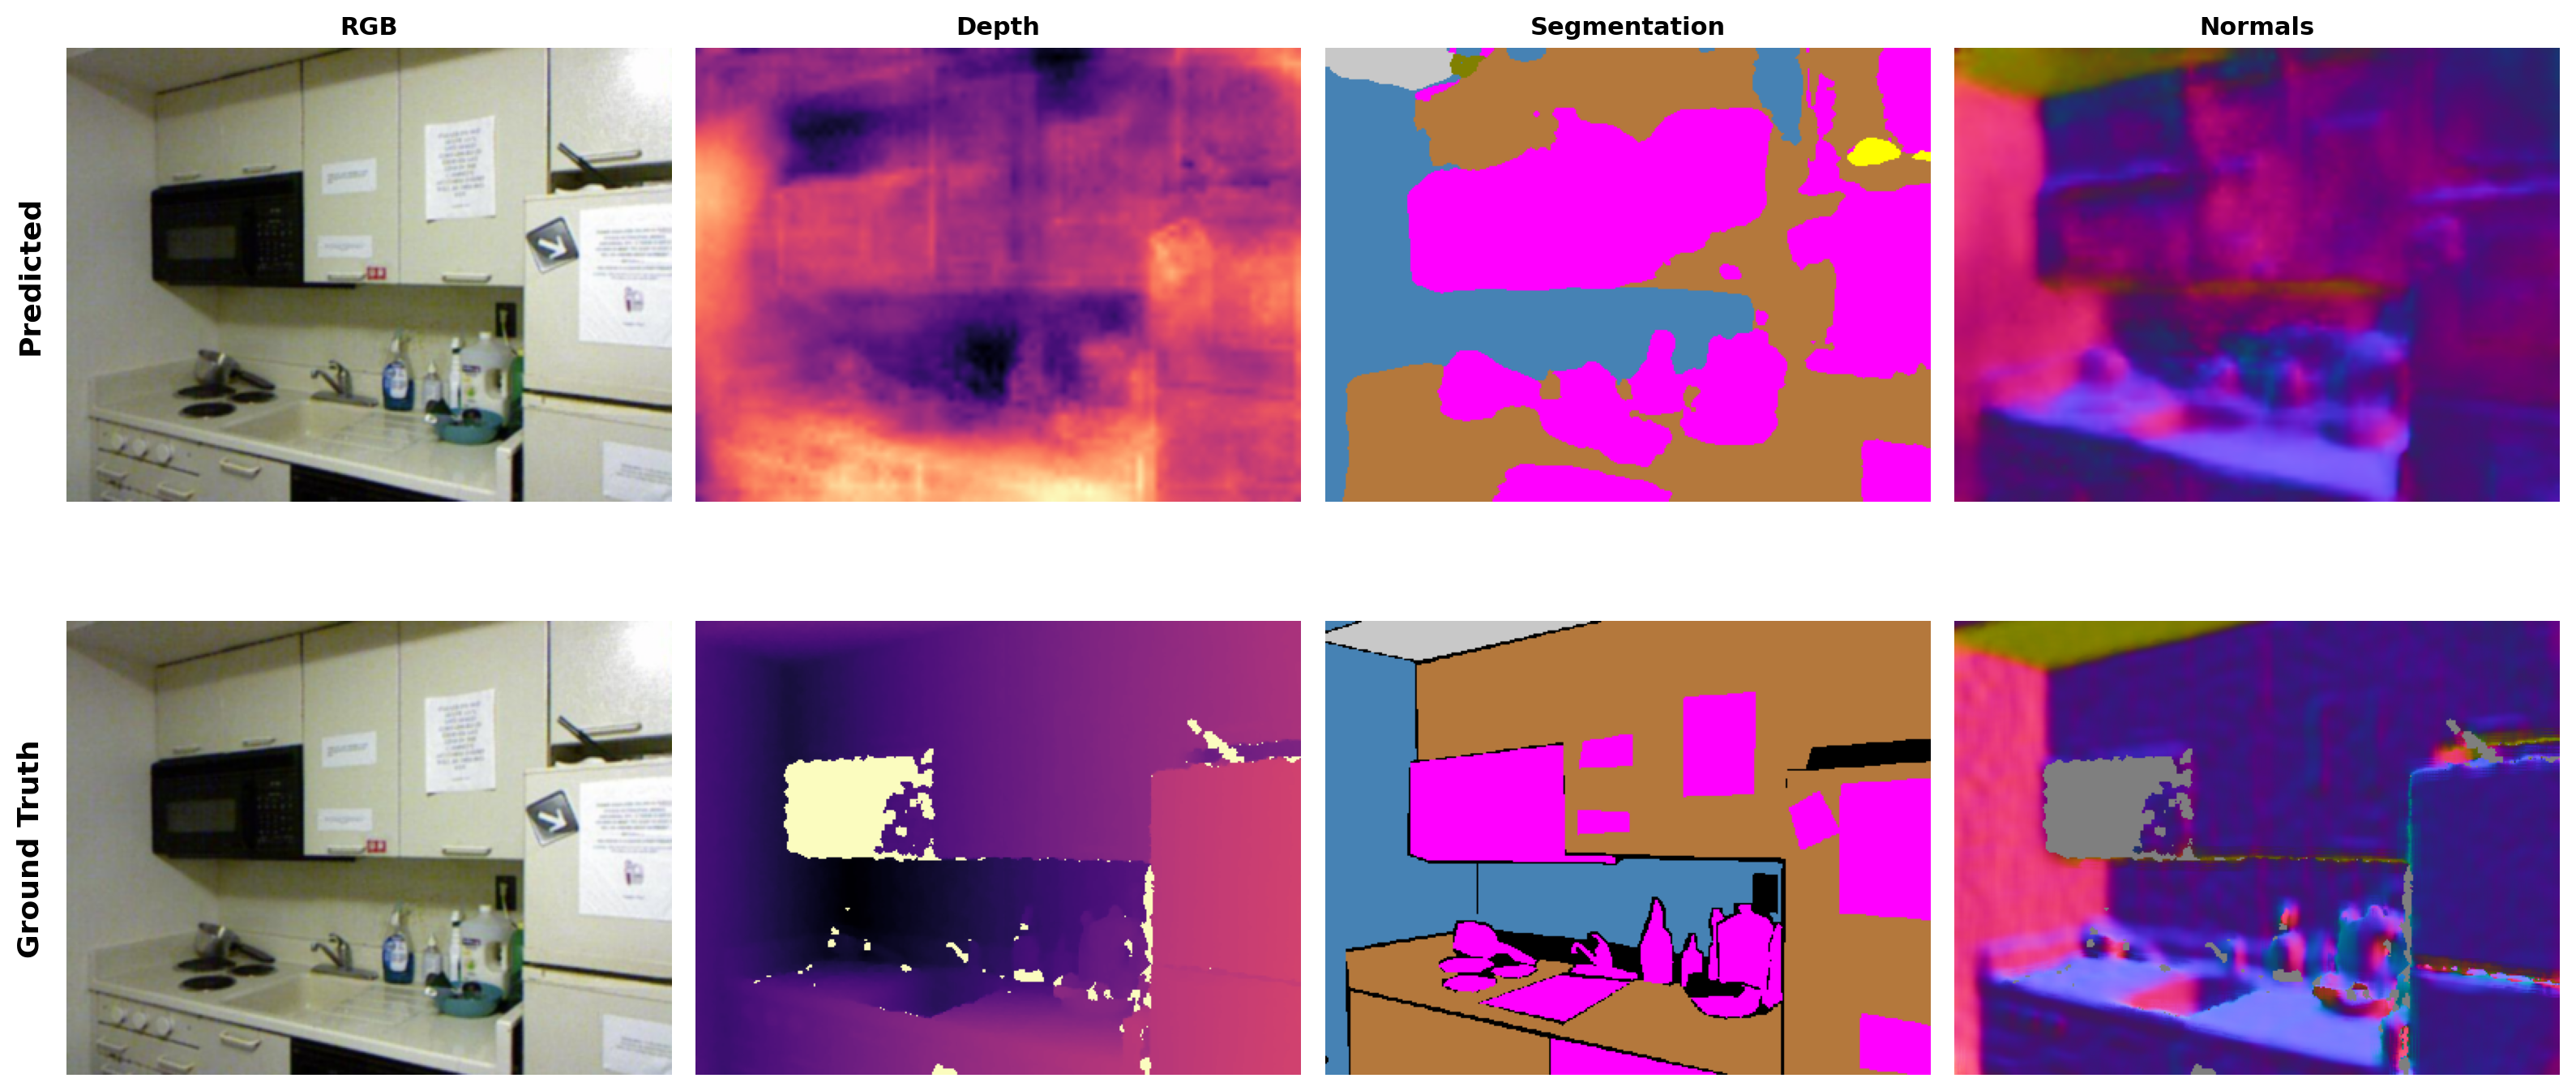
\includegraphics[width=0.48\columnwidth]{eval_results/nyuv2/visualisations/sample_0001.png} \\[2pt]
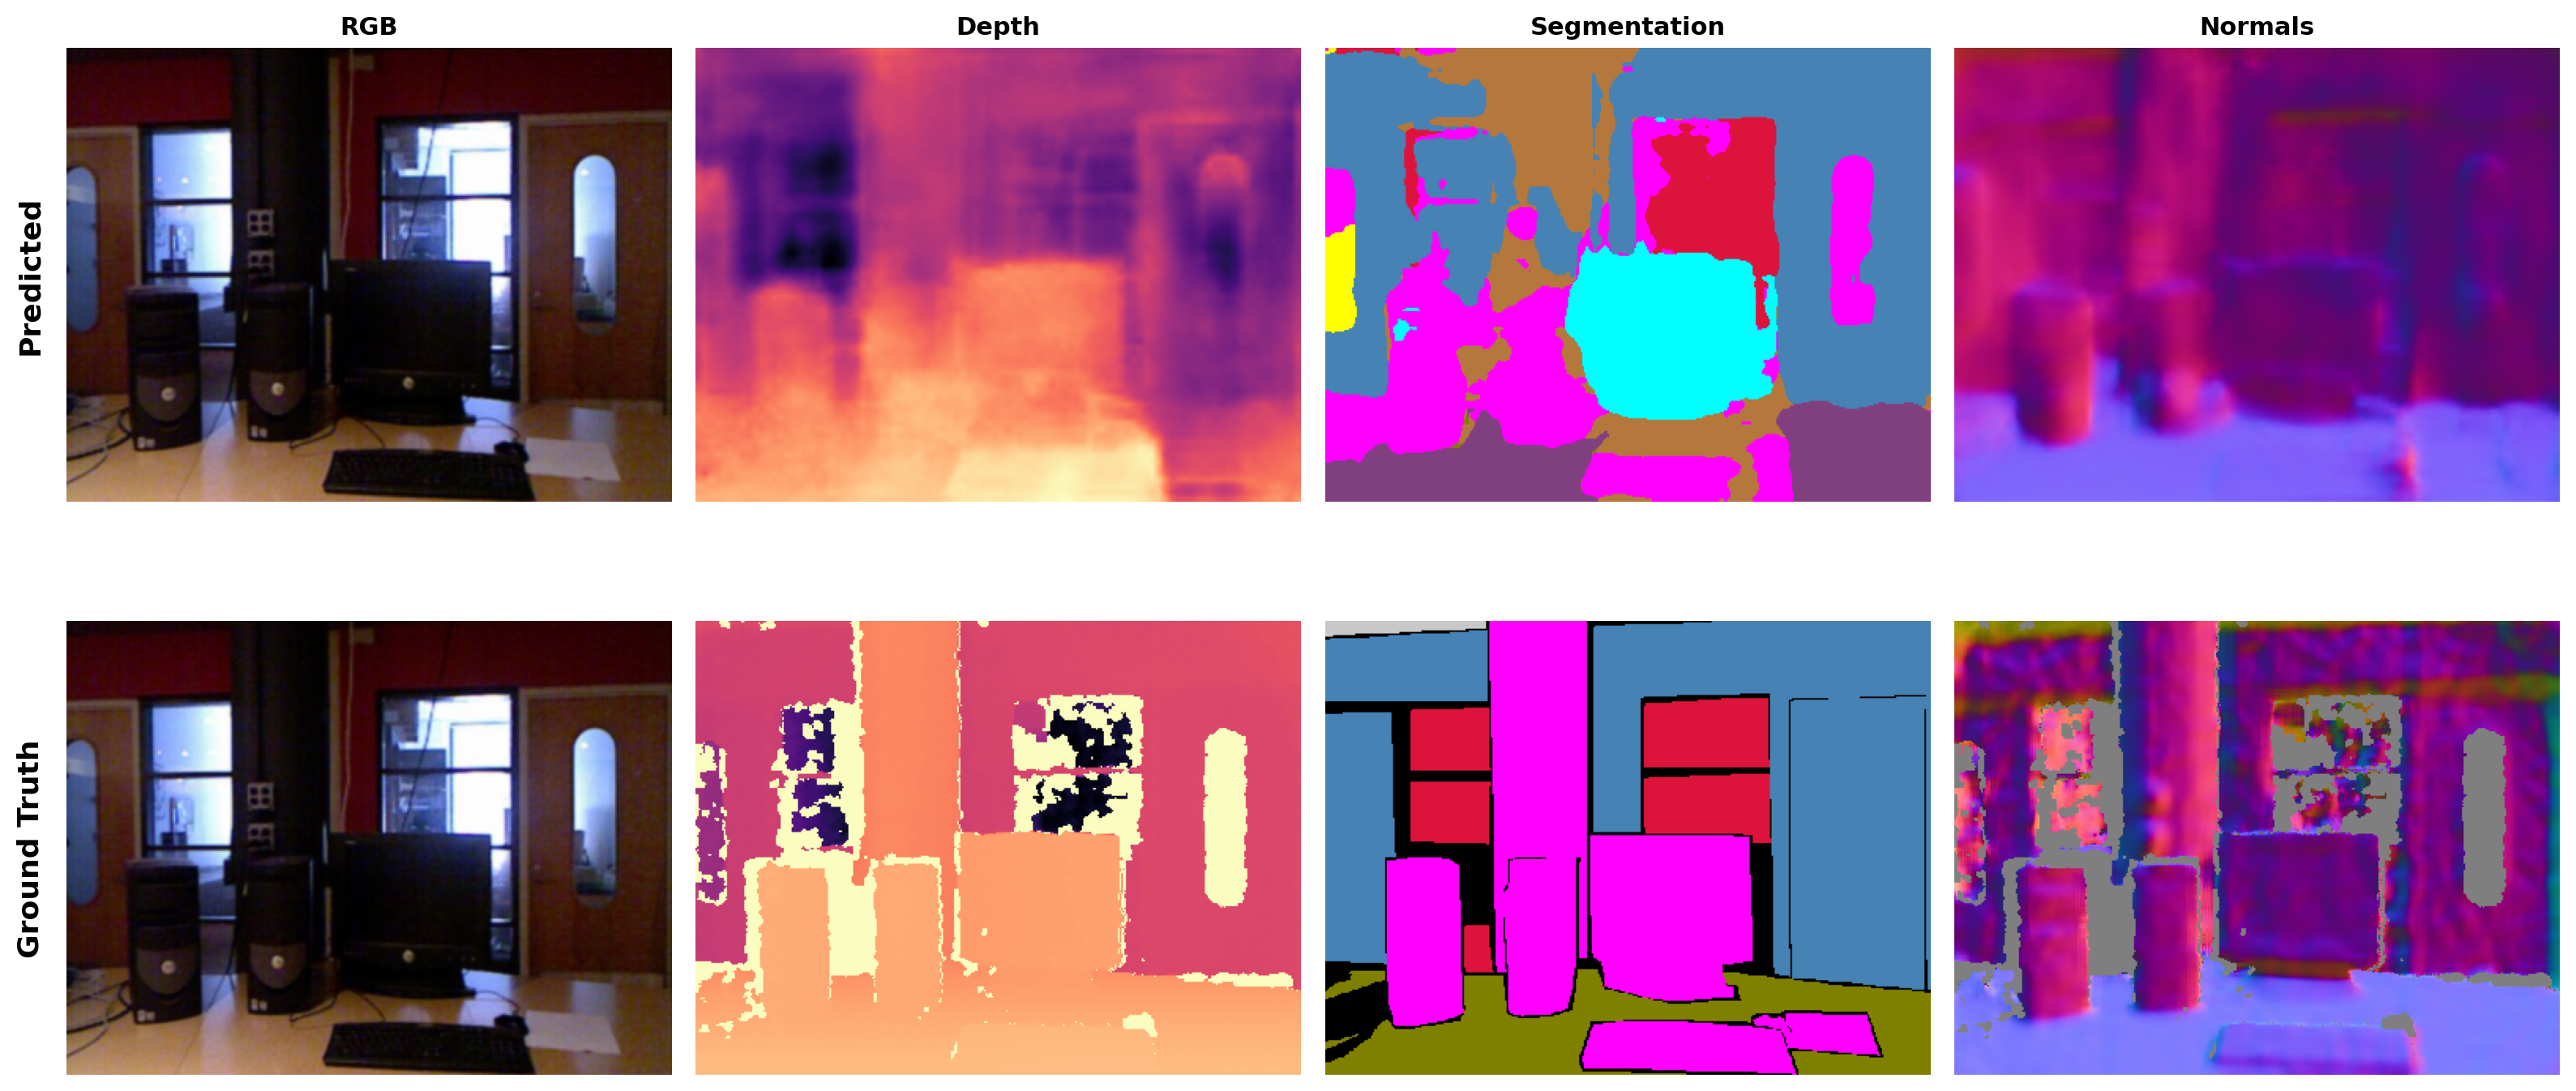
\includegraphics[width=0.48\columnwidth]{eval_results/nyuv2/visualisations/sample_0002.png} &
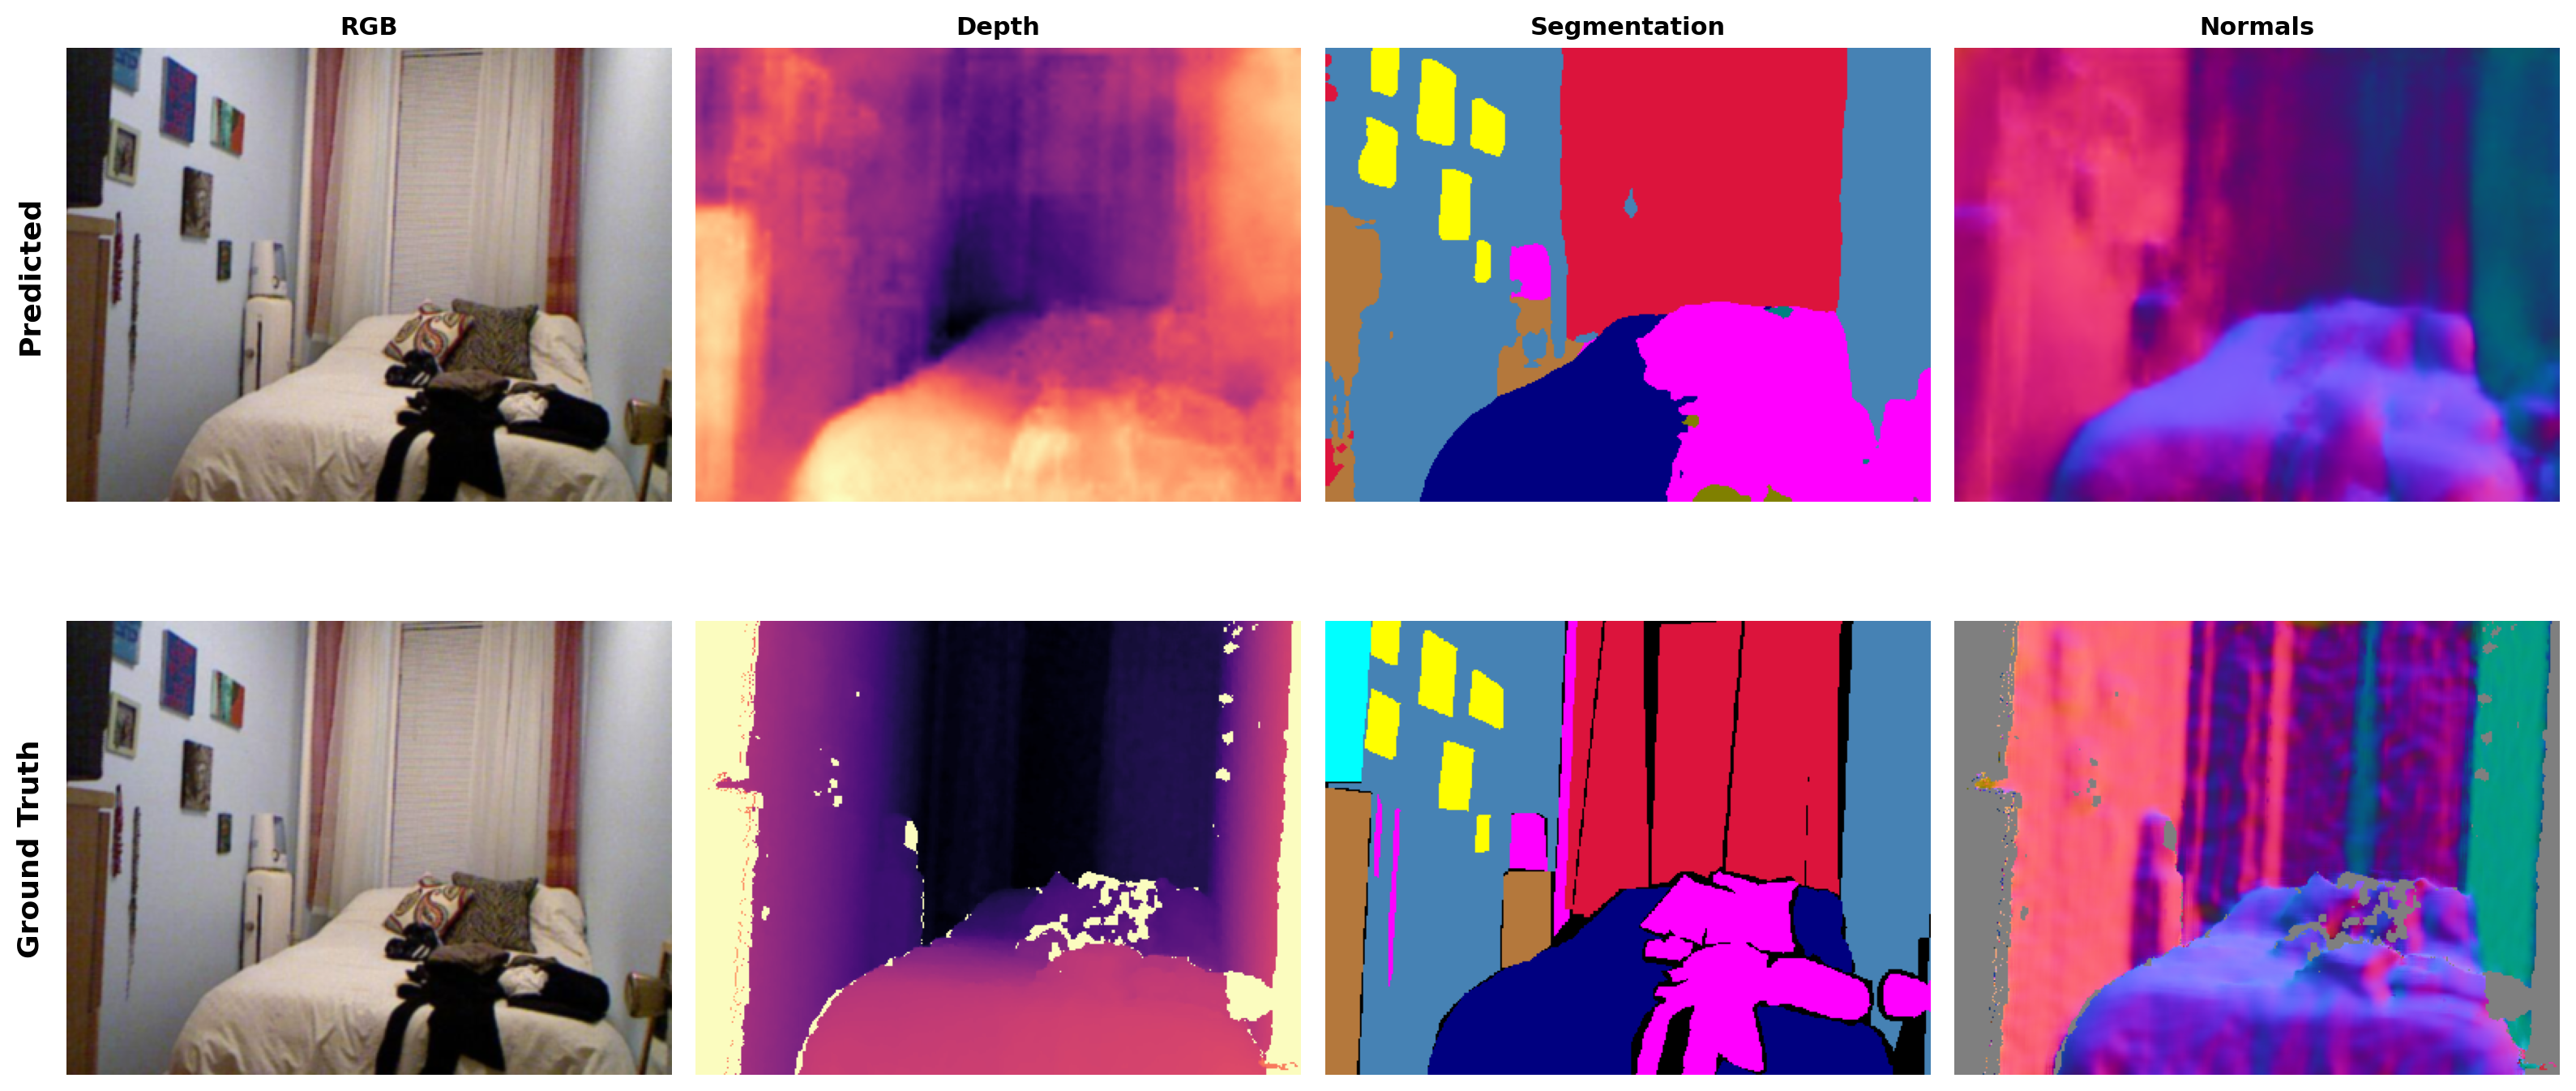
\includegraphics[width=0.48\columnwidth]{eval_results/nyuv2/visualisations/sample_0003.png} \\
\end{tabular}
\caption{Qualitative predictions on NYUv2 validation images. Each panel shows (top row) input RGB, predicted depth, predicted segmentation, and predicted surface normals; (bottom row) corresponding ground truth. The normals look visibly sharper here than on Cityscapes, likely because of the better sensor ground truth.}
\label{fig:qualitative_nyuv2}
\end{figure}

Fig.~\ref{fig:qualitative} shows some example predictions on Cityscapes. The depth maps pick up the relative ordering of objects pretty well, segmentation boundaries look clean and the normals capture the main planar orientations of roads and buildings.

Fig.~\ref{fig:qualitative_nyuv2} has the corresponding NYUv2 examples. The model handles complex indoor scenes with different viewpoints and lighting conditions reasonably well. One thing that stands out is that the normal predictions look noticeably sharper on NYUv2 than on Cityscapes which again points to the benefit of having real sensor ground truth for training.

% === CONCLUSION ===
\FloatBarrier
\section{Conclusion}

In this paper we presented MTAN-Lite, a lightweight multi-task network that predicts monocular depth, semantic segmentation, and surface normals from a single RGB image. By swapping out the heavy backbone for MobileNetV3-Large and using reduced-dimensionality attention modules, we bring the parameter count down by 81\% compared to the original MTAN, while handling three tasks on both outdoor and indoor datasets.

On Cityscapes, the model gets 70.1\% mIoU (19-class), 84.9\% $\delta_1$ for depth, and 49.1$^\circ$ normal MAE at 39.6 FPS on a GTX 1650. On NYUv2, we get 51.7\% mIoU (13-class), 0.621m RMSE, and 23.9$^\circ$ normal MAE, beating both MTAN and MTI-Net with 3 to 5$\times$ fewer parameters. To our knowledge, this is the first model under 10M parameters to do three-task dense prediction on both an outdoor and indoor benchmark.

The ablation results show that multi-task learning gives a meaningful boost to segmentation (3.3\% mIoU over single-task). Our per-category normal analysis also suggests that on Cityscapes, the main limiting factor is the quality of the pseudo-ground-truth rather than the network itself, which is backed up by the much lower normal error on NYUv2 (23.9$^\circ$ vs 49.1$^\circ$) where proper sensor normals are available.

The full codebase, trained checkpoints, and evaluation scripts are available at \url{https://github.com/Sid-5137/edgelite-mtan}.

\bibliographystyle{IEEEtran}
\bibliography{references}

\end{document}
